\section{Разработка системы}
\label{sec:development}

\subsection{Используемые средства разработки}

\subsubsection{Метасистема OSTIS}

Для реализации базы знаний, на основе которой будет функциониро-
вать медицинский ассистент была использована технология OSTIS.

В технологии OSTIS (Open Semantic Technology for Intelligent Systems) используется специальный язык программирования, называемый SC-код (Semantic Code).
 
SC-код– способ универсального смыслового представления (кодирования) информации в памяти компьютерных систем. Он основан на теории графов (синтаксис) и теории множеств (семантика), что обеспечивает универсальность и унифицированность (единообразие) представления информации,
удобство машинной обработки и восприятия человеком. 

С помощью SC-кода можно описывать базы знаний, решатели задач и интерфейс интеллектуальной системы.

SC-код - это компьютерный код семантических сетей, являющий-
ся упрощенным представлением семантических сетей – с минимальным
алфавитом и бинарными связками.

SC-code является абстрактным языком, но его можно визуализировать в различных формах. Формы внешнего представления SC-кода: 
\begin{itemize}
    \item SCs (текстовый линейный)
    \item SCn (гипертекстовый)
    \item SCg (графический)
\end{itemize}

Для описания понятий использовался подъязык SC-кода - SCg.

SCg (Semantic Code graphical) является частью технологии OSTIS и представляет собой графический язык для описания знаний и моделирования визуальных структур.

SCg используется для визуального представления знаний, сущностей, связей и операций в виде графов. Он предоставляет графический способ описания и визуализации знаний, что делает его более доступным и интуитивно понятным для пользователей, не имеющих опыта в программировании.

Особенность SCg:

Узлы (Nodes). Узлы в SCg представляют собой сущности или объекты, которые могут быть описаны с помощью SC кода. Каждый узел имеет определенный тип и характеристики, которые могут быть заданы с использованием атрибутов.

SCg является удобным инструментом для визуализации и моделирования знаний в технологии OSTIS. Он позволяет легко создавать и взаимодействовать с графическими структурами знаний, что делает его полезным для разработки интеллектуальных систем и решения сложных задач.

Для создания базы знаний в SCg коде использовался инструмент KBE.

KBE (Knowledge Base Editor) - это инструмент для создания фрагментов базы знаний (БЗ) в SCg (Semantic Code graph). SCg - это формальный язык для описания знаний с использованием семантической графики. KBE предоставляет пользователю графический интерфейс для создания и редактирования знаний в виде семантических графов.

Основные возможности KBE включают:
\begin{itemize}
    \item Графический интерфейс. KBE предоставляет интуитивно понятный графический интерфейс, который позволяет пользователям визуализировать и редактировать семантические графы. Это облегчает создание и редактирование структуры базы знаний.
    \item Визуализация. KBE предоставляет средства для визуализации семантических графов, что помогает пользователям лучше понять структуру и связи между знаниями в базе данных.
\end{itemize}

Благодаря KBE пользователи могут легко создавать и управлять базами знаний в SCg, что делает процесс разработки и использования семантических моделей более эффективным и удобным.

\subsubsection{Docker}

Docker — это открытая платформа для разработки, доставки и запуска приложений. Docker предоставляет возможность упаковать и запустить приложение в слабо изолированной среде, называемой контейнером. Преимуществами Docker являются:
\begin{itemize}
    \item Платформенная независимость– приложение, контейнеризированное при помощи Docker возможно развернуть и запустить на всех наиболее популярных плафтормах.
    \item Контейнеры легковесны и содержат в себе все необходиое для запуска приложения: операционную систему, программное обеспечение, библиотеки, конфигурацию.
    \item Удобство распространения и совместного использования контейнеров.
\end{itemize}

\subsubsection{Python}

Python — это интерпретируемый высокоуровневый язык программирования с динамической типизацией. Его основными особенностями являются простота синтаксиса и широкий выбор библиотек для различных областей разработки, что делает его универсальным инструментом как для новичков, так и для профессионалов. Python активно применяется в веб-разработке, анализе данных, машинном обучении, разработке искусственного интеллекта, автоматизации процессов и научных исследованиях.

Основные преимущества Python:
\begin{itemize}
    \item Простота и читаемость кода — благодаря лаконичному синтаксису и понятной структуре, код на Python легко поддерживать и расширять.
    \item Кроссплатформенность — Python может быть установлен и запущен на различных операционных системах, таких как Windows, macOS и Linux.
    \item Большое сообщество и обширная стандартная библиотека — Python имеет большое сообщество разработчиков и богатую библиотеку, которая поддерживает широкий спектр задач и позволяет быстро находить и исправлять ошибки.
    \item Поддержка множества библиотек и фреймворков — для Python существует большое количество готовых библиотек и фреймворков, таких как Django и Flask для веб-разработки, NumPy и Pandas для анализа данных, TensorFlow и PyTorch для машинного обучения.
\end{itemize}


\subsection{Демонстрация базы знаний}

Исходя из процесса разработки агента-решателя задач диагностики по симптомам, в базе знаний интеллектуальной системы был выявлен ряд неточностей при описании симптоматики болезней, в следствие чего агент-решатель не имел возможности корректно диагностировать некоторые болезни. По этой причине был проведен аудит базы знаний интеллектуальной системы и скорректировано описание симптоматики под единый шаблон у ряда болезней Общее количество фрагментов базы знаний, подвергаемых проверке, составило более 150 единиц.

Ниже представлены примеры формализации основных понятий.


На рис. \hyperref[метка2]{3.1} пример определения болезни.

\begin{figure}[H]
    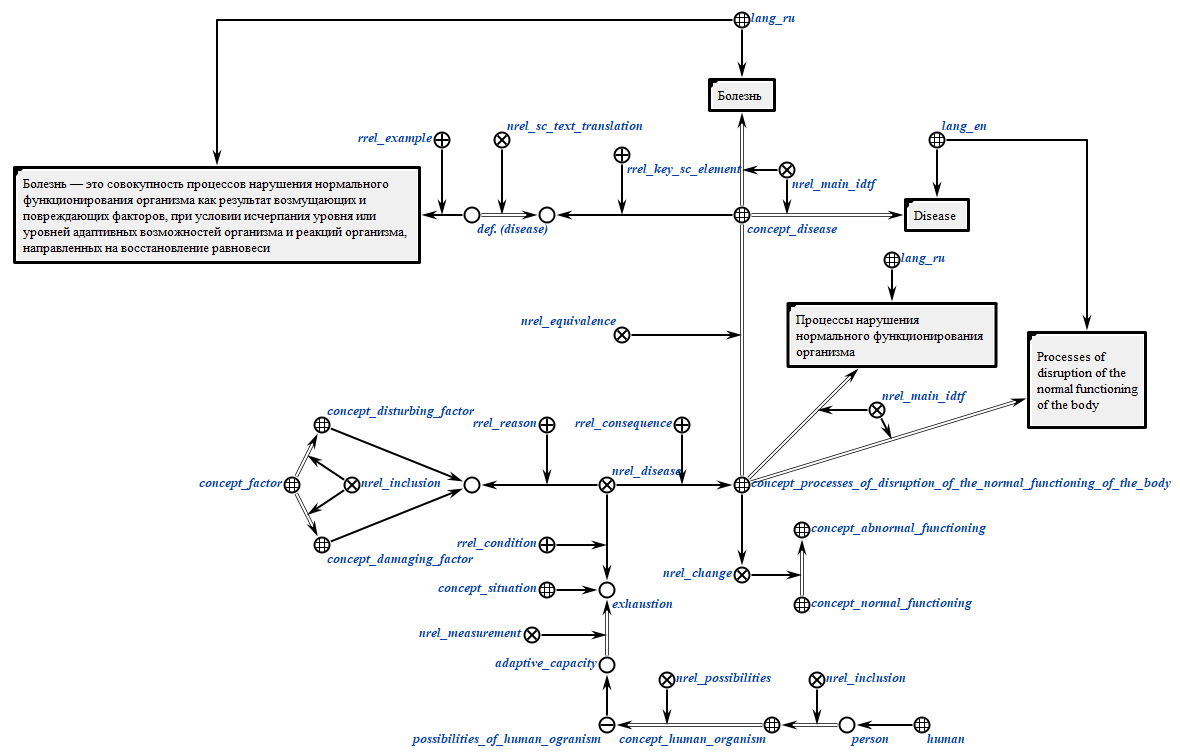
\includegraphics[width=0.8\textwidth]{sections/disease_def.png}
    \caption{Определение болезни}
    \label{метка2}
\end{figure}

На рис. \hyperref[метка3]{3.2} пример погружения в систему понятия болезнь.

\begin{figure}[H]
    \centering
    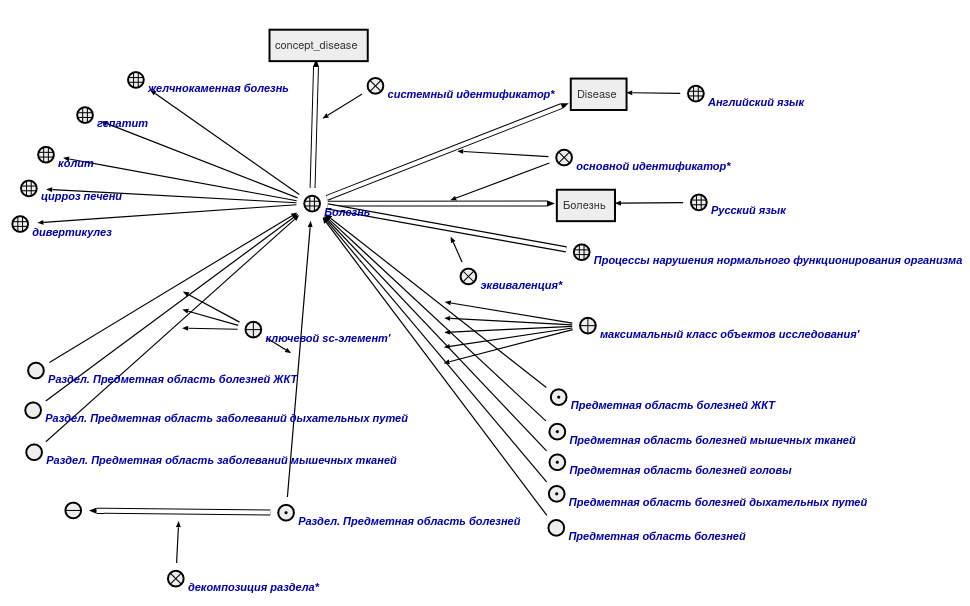
\includegraphics[width=0.8\textwidth]{sections/disease.png}
    \caption{Определение болезни в системе}
    \label{метка3}
\end{figure}


На рис. \hyperref[метка4]{3.3} пример определения понятия кашель.
\begin{figure}[H]
    \centering
    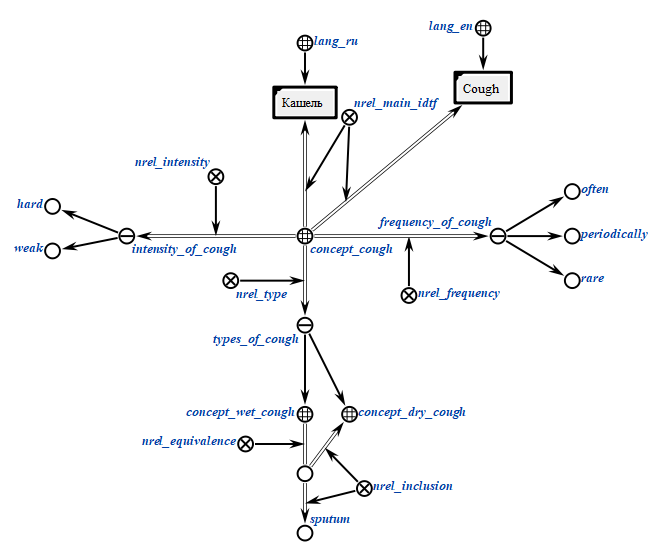
\includegraphics[width=0.8\textwidth]{sections/cough_def.png}
    \caption{Определение кашля}
    \label{метка4}
\end{figure}

На рис. \hyperref[метка5]{3.4} пример погружения в систему понятия кашель.

\begin{figure}[H]
    \centering
    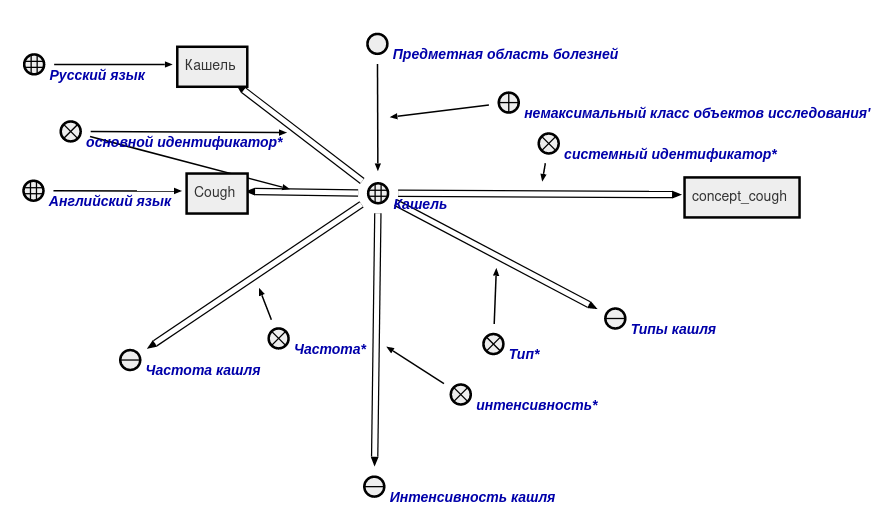
\includegraphics[width=0.8\textwidth]{sections/cough.png}
    \caption{Определение кашля в системе}
    \label{метка5}
\end{figure}



На рис. \hyperref[метка6]{3.5} пример отображения предметной области\hyperref[метка7]{(а)} и раздела предметной области\hyperref[метка8]{(б)} в системе.

\begin{figure}[h]
    \centering
    \begin{subfigure}{0.45\textwidth}
        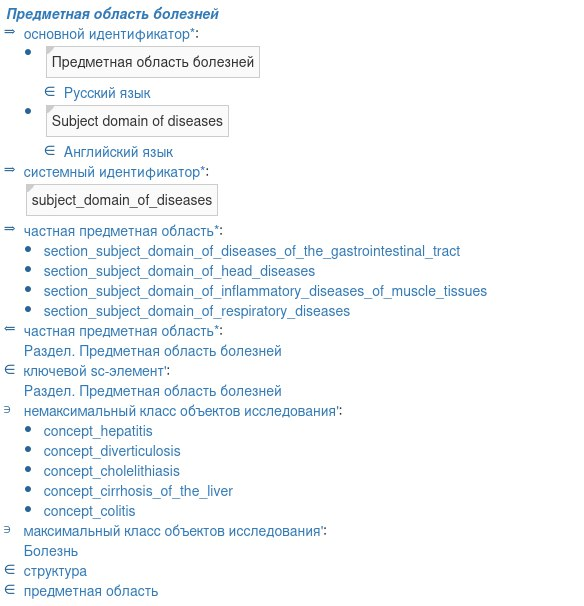
\includegraphics[height=8cm]{sections/sub_dom_disease.jpg}
        \caption{Предметная область болезней}
        \label{метка7}
    \end{subfigure}
    \hfill
    \begin{subfigure}{0.45\textwidth}
        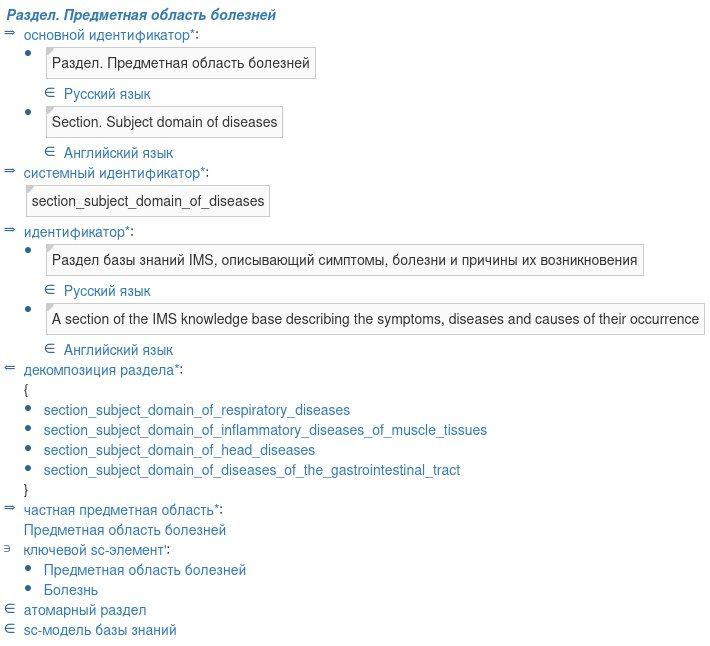
\includegraphics[height=8cm]{sections/sec_sub_dom_disease.jpg}
        \caption{Раздел. Предметная область болезней}
        \label{метка8}
    \end{subfigure}
    \caption{Пример погруженной в систему предметной области}
    \label{метка6}
\end{figure}

\newpage

\subsection{Демонстрация и тестирование агента анализа крови}

На рисунке \hyperref[запуск]{3.6} представлен пример входной структуры для агента диагностики по симптомам:
\begin{figure}[H]
    \centering
    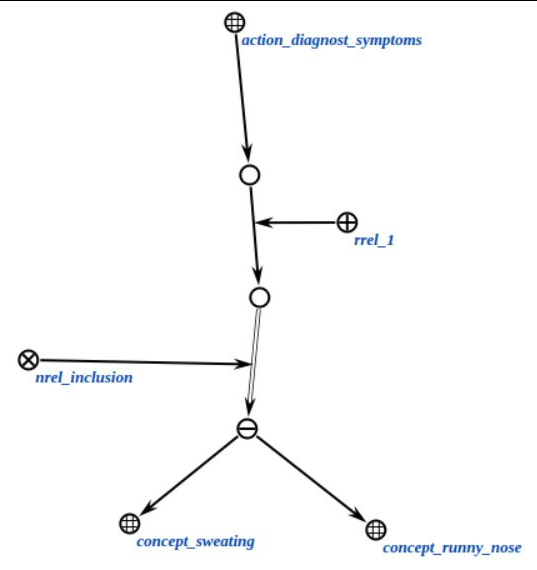
\includegraphics[width=0.5\textwidth]{sections/diagnostic_entry.png}
    \caption{Пример входной структуры}
    \label{запуск}
\end{figure}

На рисунке \hyperref[результат]{3.7} представлен результат работы данного агента:
\begin{figure}[H]
    \centering
    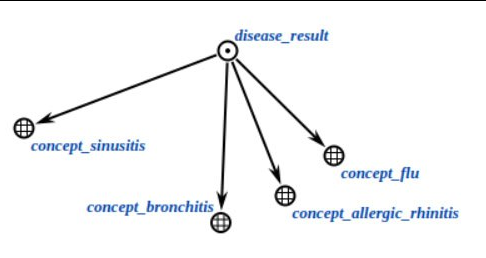
\includegraphics[width=0.8\linewidth]{sections/diagnostic_exit.png}
    \caption{Результат работы агента}
    \label{результат}
\end{figure}

На рисунке \hyperref[результат_уточнение]{3.8} представлен результат работы данного агента с информацией о количестве подходящих к конкретной болезни симптомов из входной структуры:
\begin{figure}[H]
        \centering
        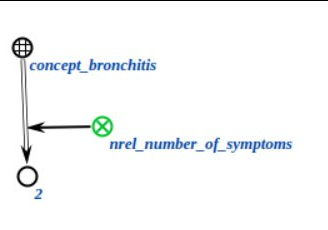
\includegraphics[width=0.5\linewidth]{sections/diagnostic_exit_specific_result.png}
        \caption{Результат работы агента при рассмотрении конкретной болезни}
        \label{результат_уточнение}
\end{figure}


\subsection{Демонстрация и тестирование веб-приложения}

На рисунках \hyperref[регистрация]{3.9} и \hyperref[авторизация]{3.10} представлены соответственно окно регистрации и окно авторизации пользователя в системе. После заполнения одного из приведённых окон и отправки пользователем данных соответствующий агент-решатель реализует процесс регистрации или авторизации пользователя в системе, предварительно проверив корректность введенных данных, а также отобразит данные в системе о результате своей работы.

\begin{figure}[H]
    \centering
    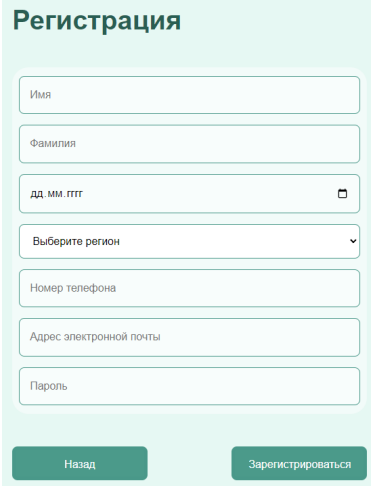
\includegraphics[width=0.6\textwidth, height=12cm]{sections/web_sign_up.PNG}
    \caption{Окно регистрации пользователя в системе}
    \label{регистрация}
\end{figure}

\begin{figure}[H]
    \centering
    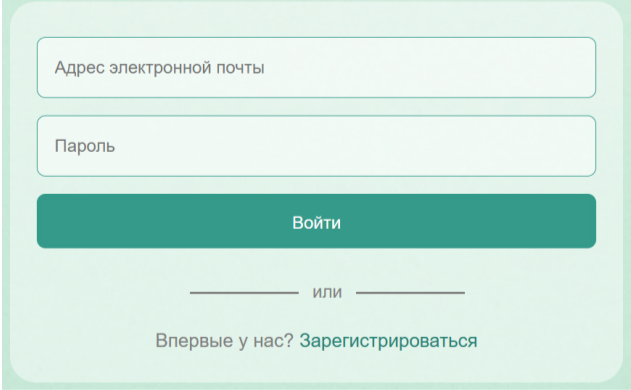
\includegraphics[width=0.6\textwidth]{sections/web_log_in.PNG}
    \caption{Окно авторизации пользователя в системе}
    \label{авторизация}
\end{figure}

На рисунках \hyperref[запись]{3.11}, \hyperref[мед_карта]{3.12} и \hyperref[история_диагностик]{3.13} представлены разработанные окна записи на прием к врачу с выбором времени и места консультации, заполнения и просмотра медицинской карты пациента, а также истории проводимых ранее в системе диагностик с результатами и временем соответственно. 

\begin{figure}[H]
    \centering
    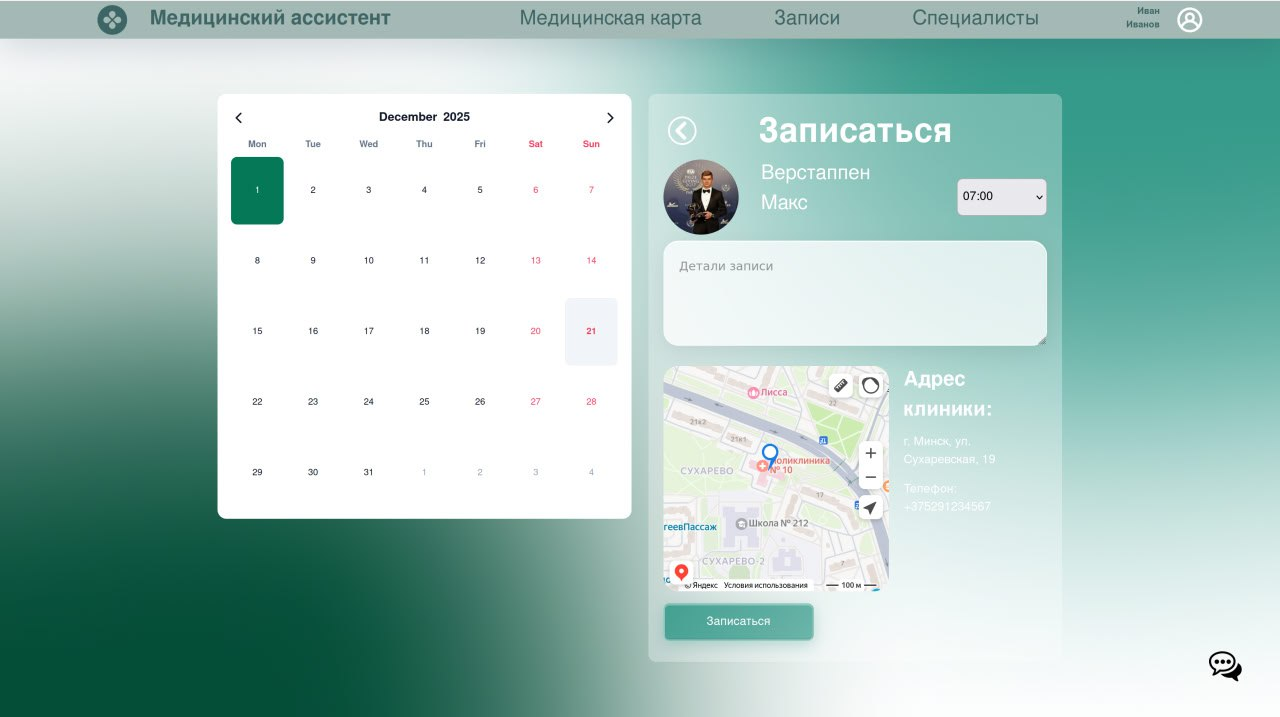
\includegraphics[width=0.9\textwidth]{sections/booking_to_doctor.png}
    \caption{Окно записи на прием}
    \label{запись}
\end{figure}

\begin{figure}[H]
    \centering
    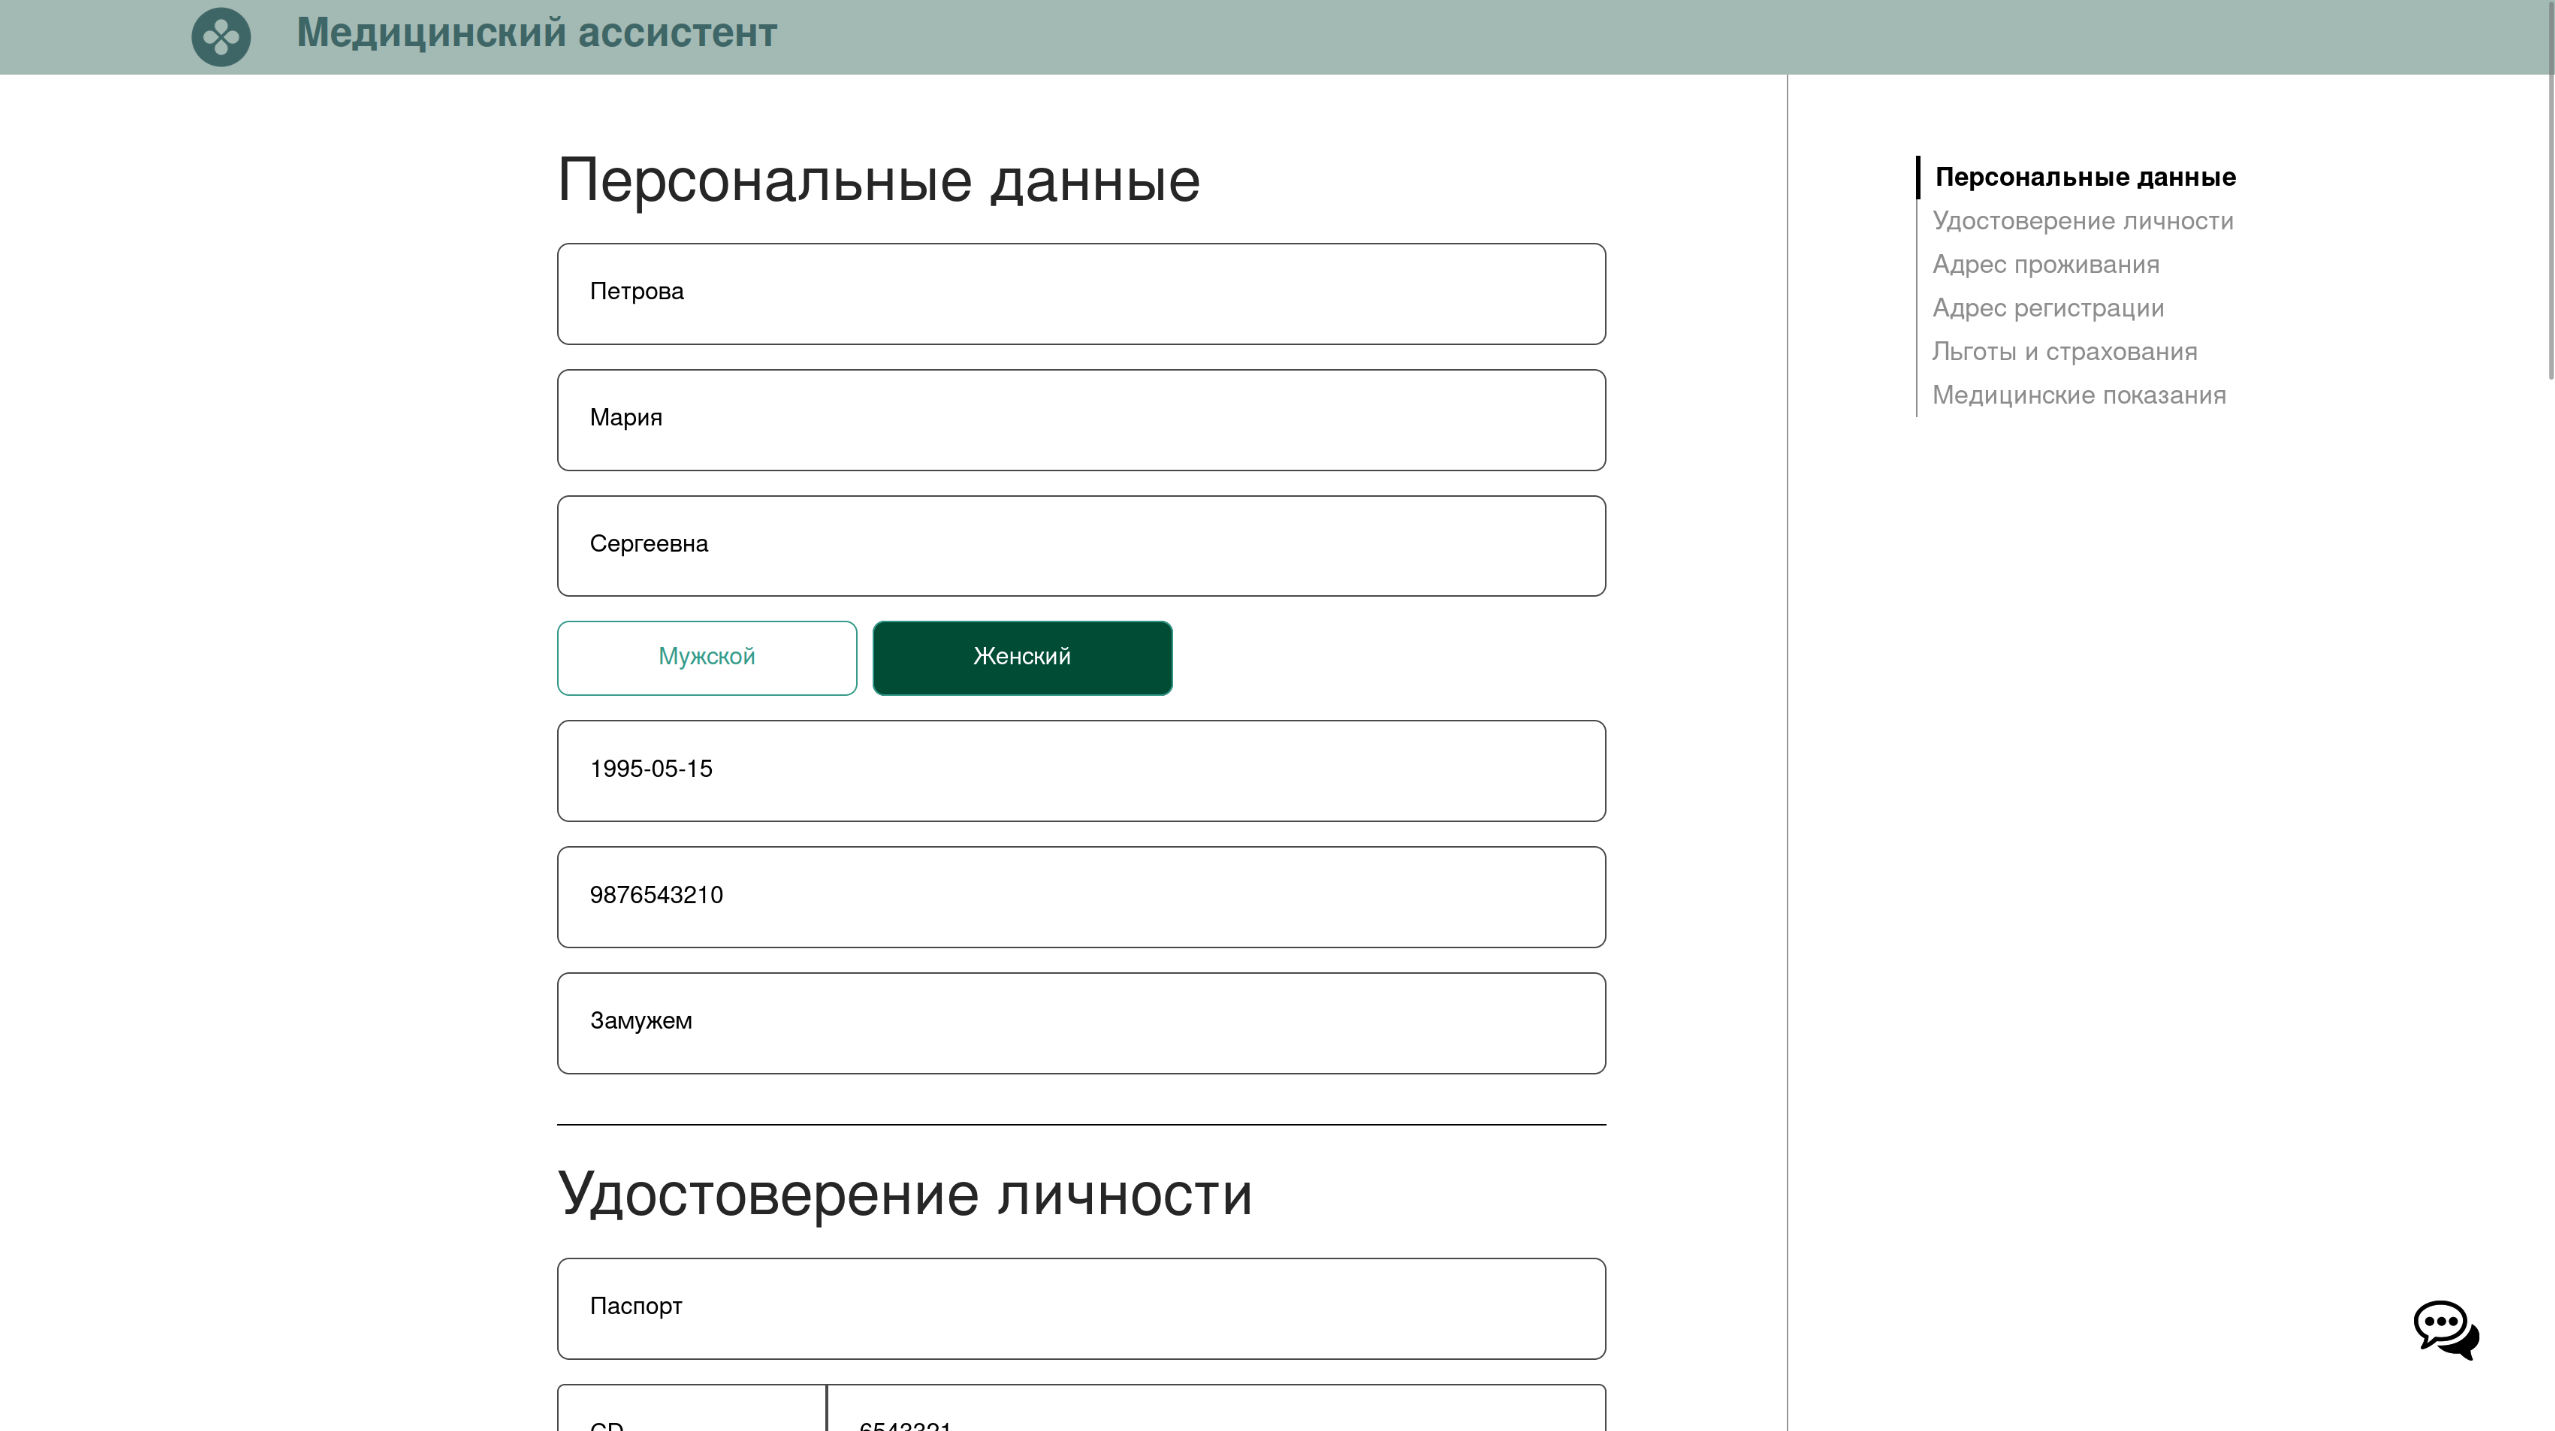
\includegraphics[width=0.9\textwidth]{sections/med_card.png}
    \caption{Окно заполнения и отображения медицинской карты}
    \label{мед_карта}
\end{figure}

\begin{figure}[H]
    \centering
    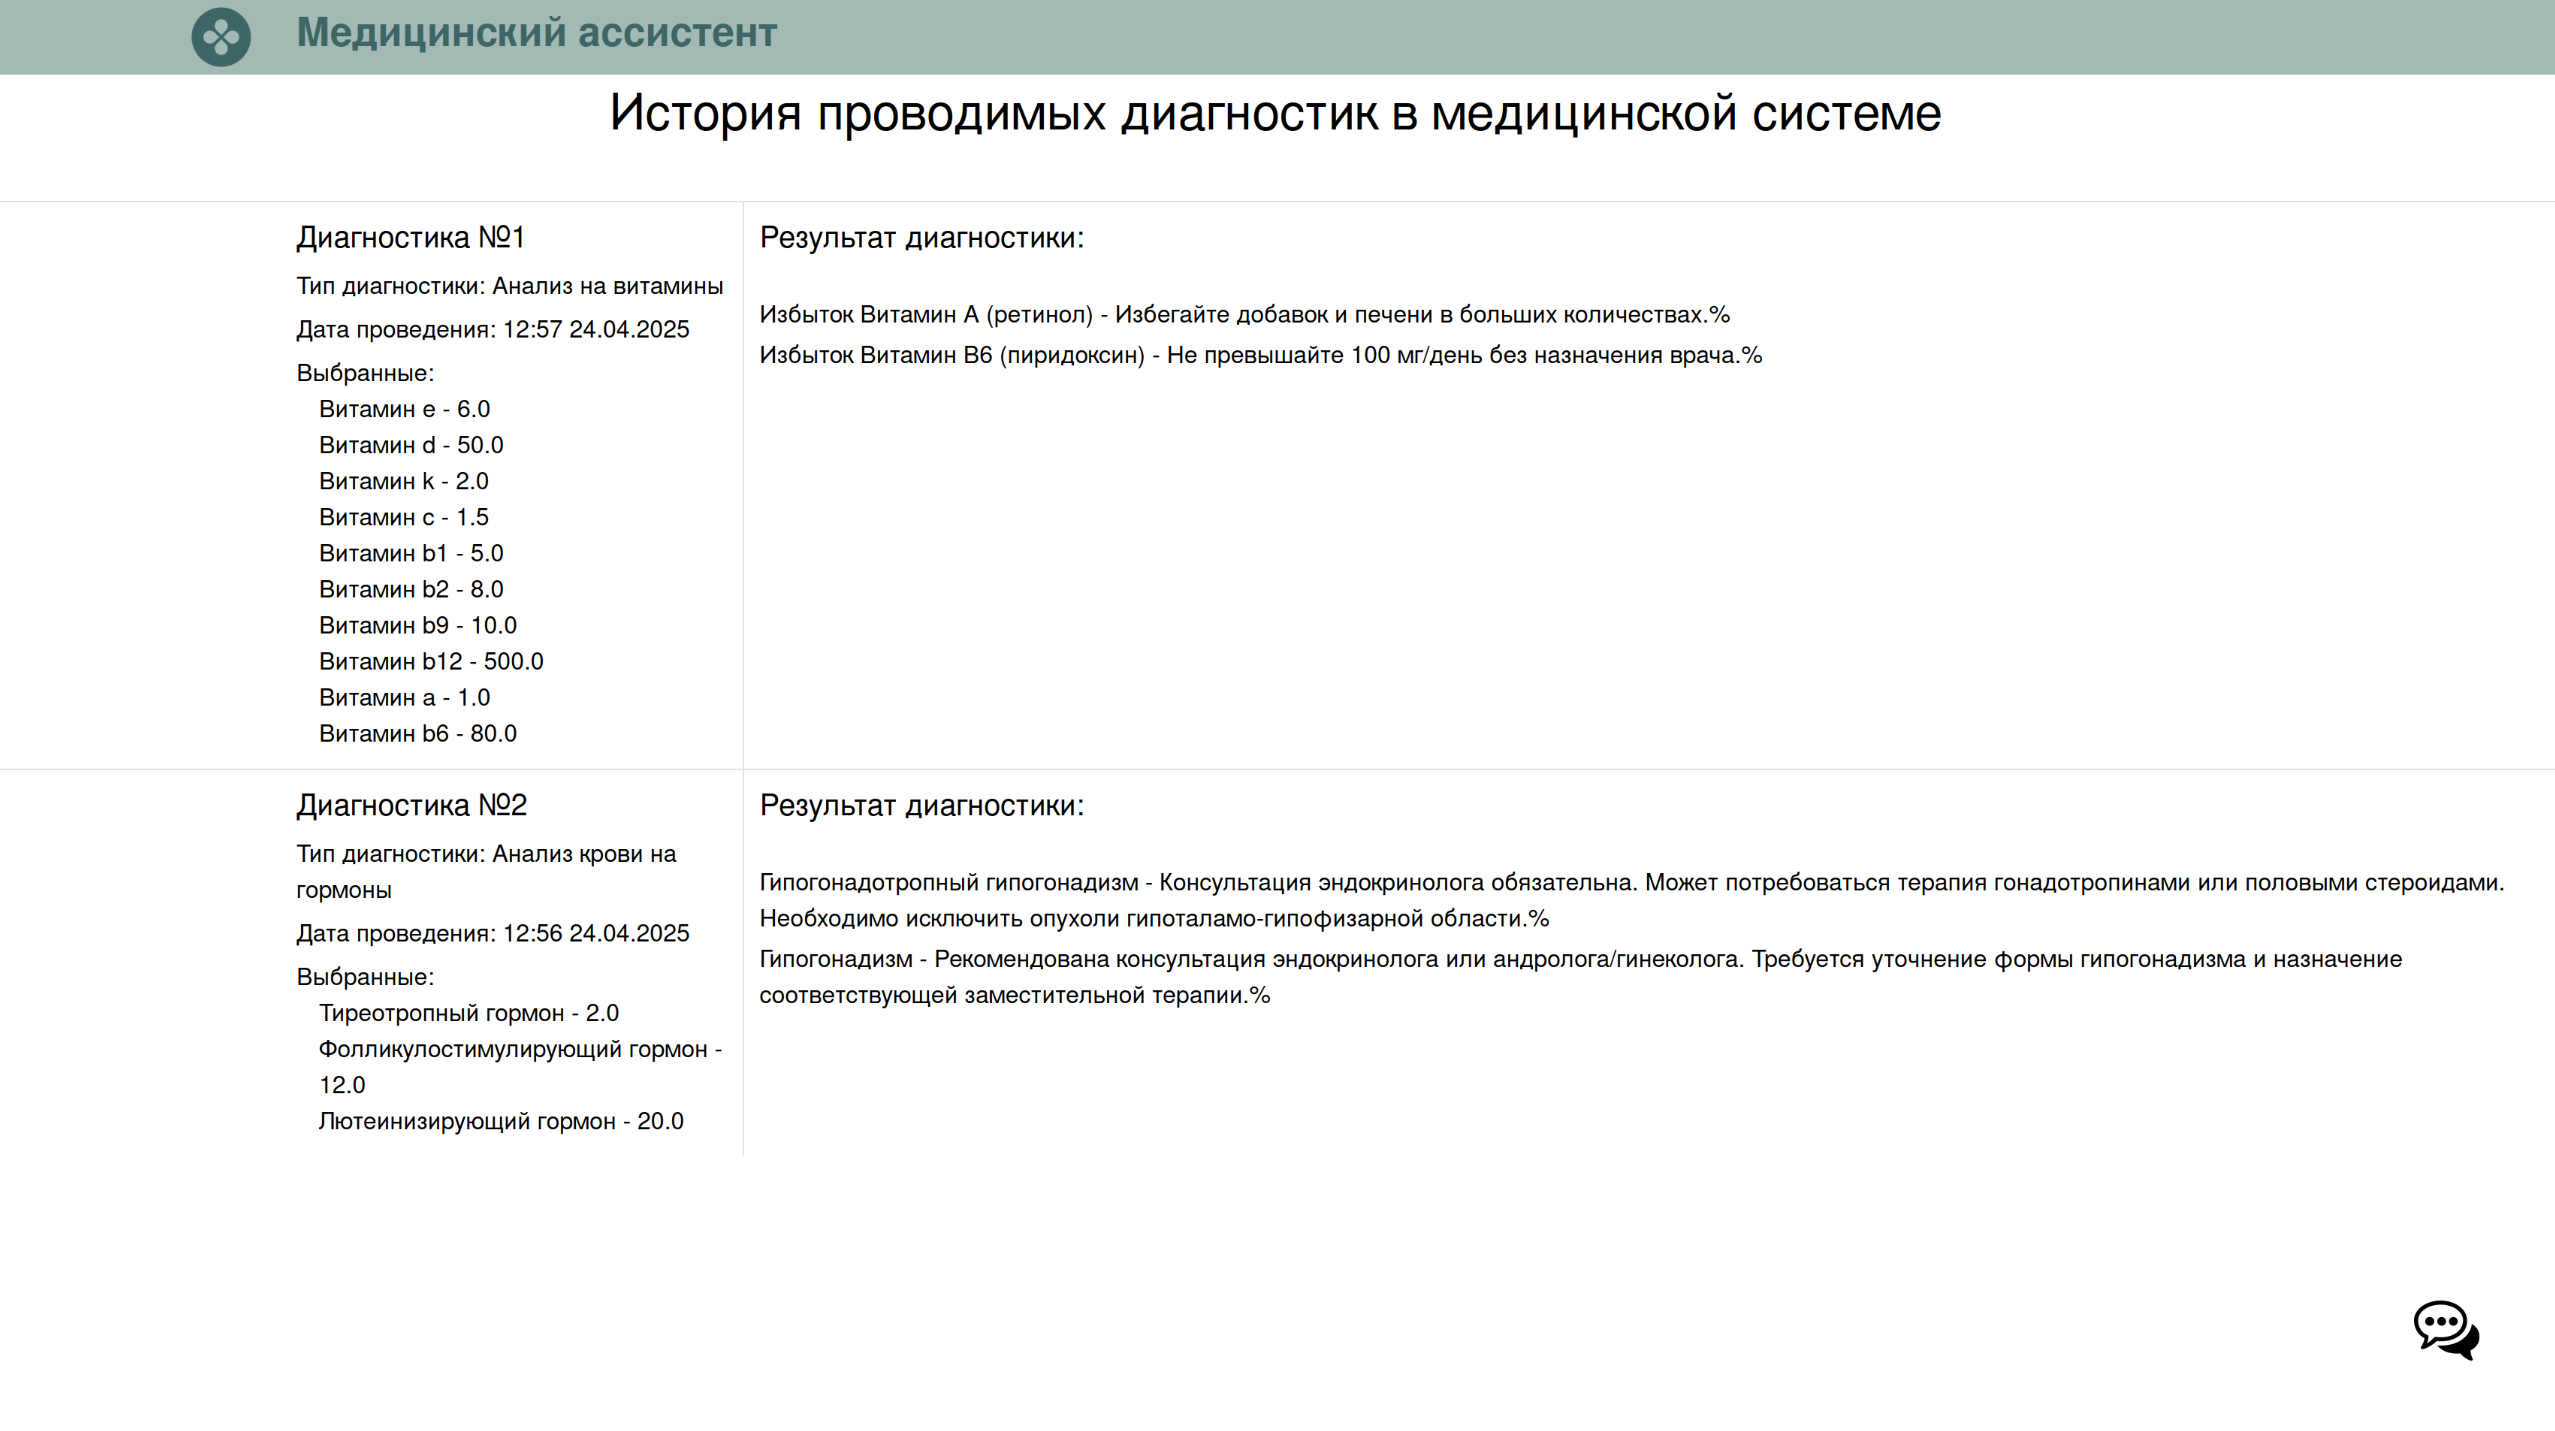
\includegraphics[width=0.9\textwidth]{sections/history_of_diagnostic.png}
    \caption{Окно с историей проводимых в системе диагностик}
    \label{история_диагностик}
\end{figure}

Также были разработаны и интегрированы в веб-приложение страницы и агенты для прохождения диагностики по специальным анализам крови, по симптомам, а также навигации на базе знаний и рекомендаций по здоровью. Примеры на рисунках \hyperref[кровь]{3.14}, \hyperref[кровь_результат]{3.15}, \hyperref[симптомы]{3.16}, \hyperref[симптомы_рузультат]{3.17} и \hyperref[навигация]{3.18}.

\begin{figure}[H]
    \centering
    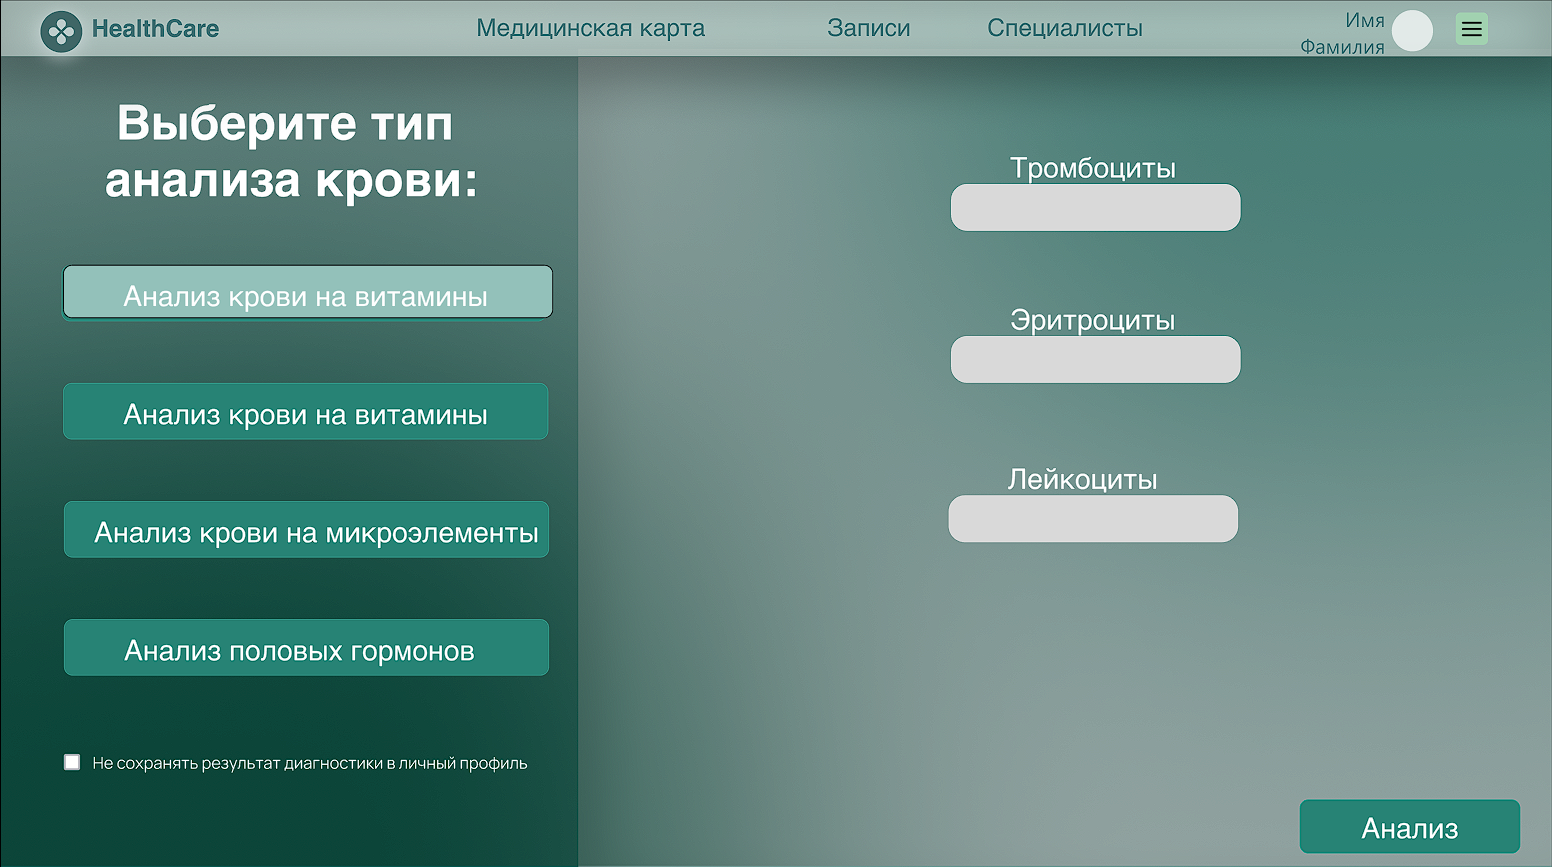
\includegraphics[width=0.9\textwidth]{sections/gormon_blood_test.png}
    \caption{Окно диагностики по результатам гормонального анализа крови}
    \label{кровь}
\end{figure}

\begin{figure}[H]
    \centering
    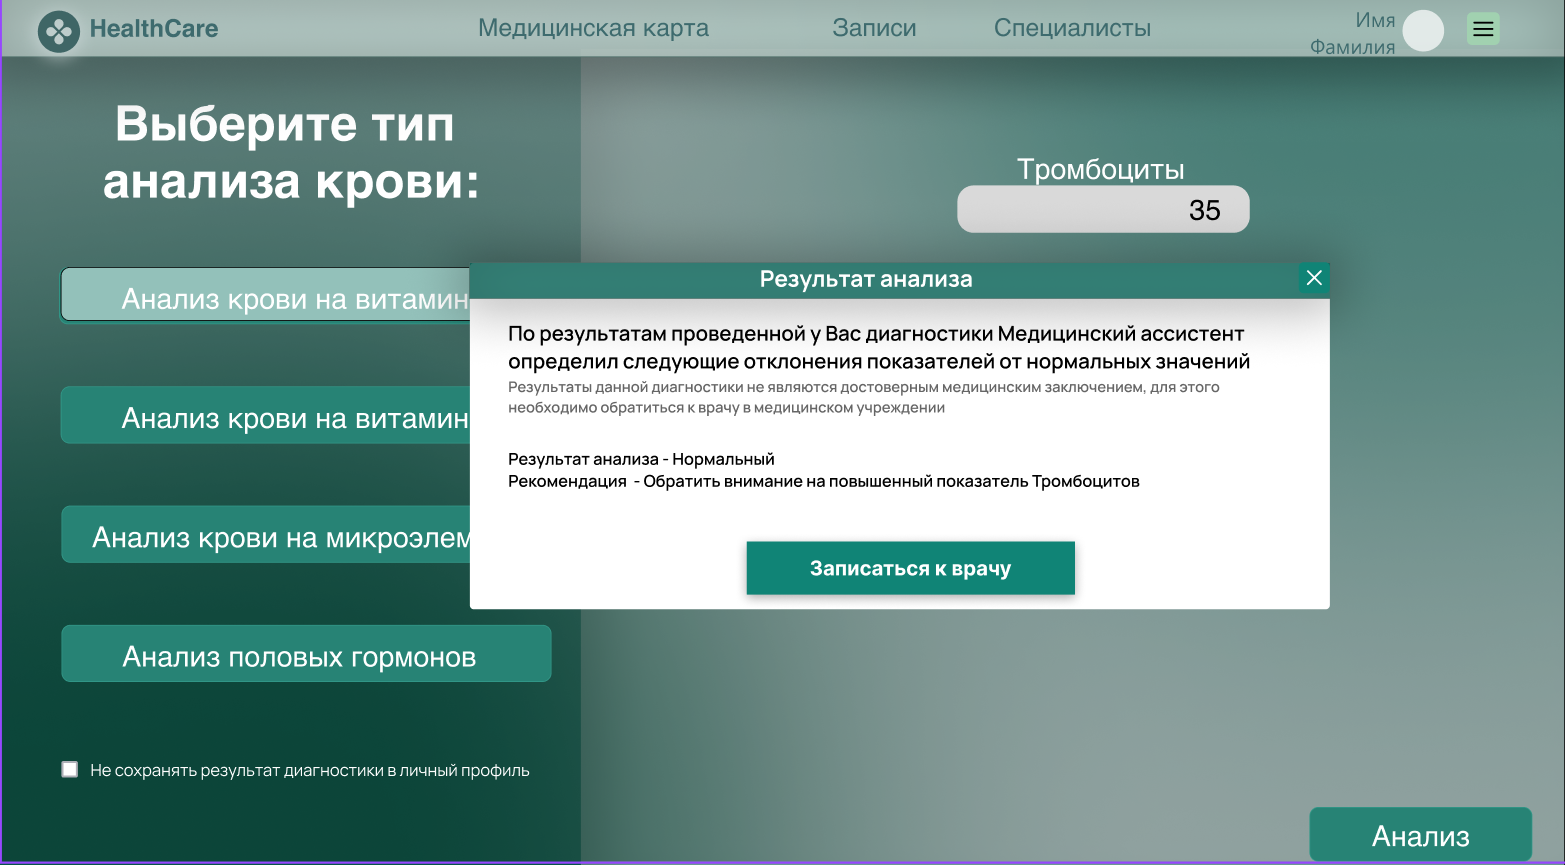
\includegraphics[width=0.9\textwidth]{sections/gormon_blood_result.png}
    \caption{Окно результата диагностики по гормональному анализу крови}
    \label{кровь_результат}
\end{figure}

\begin{figure}[H]
    \centering
    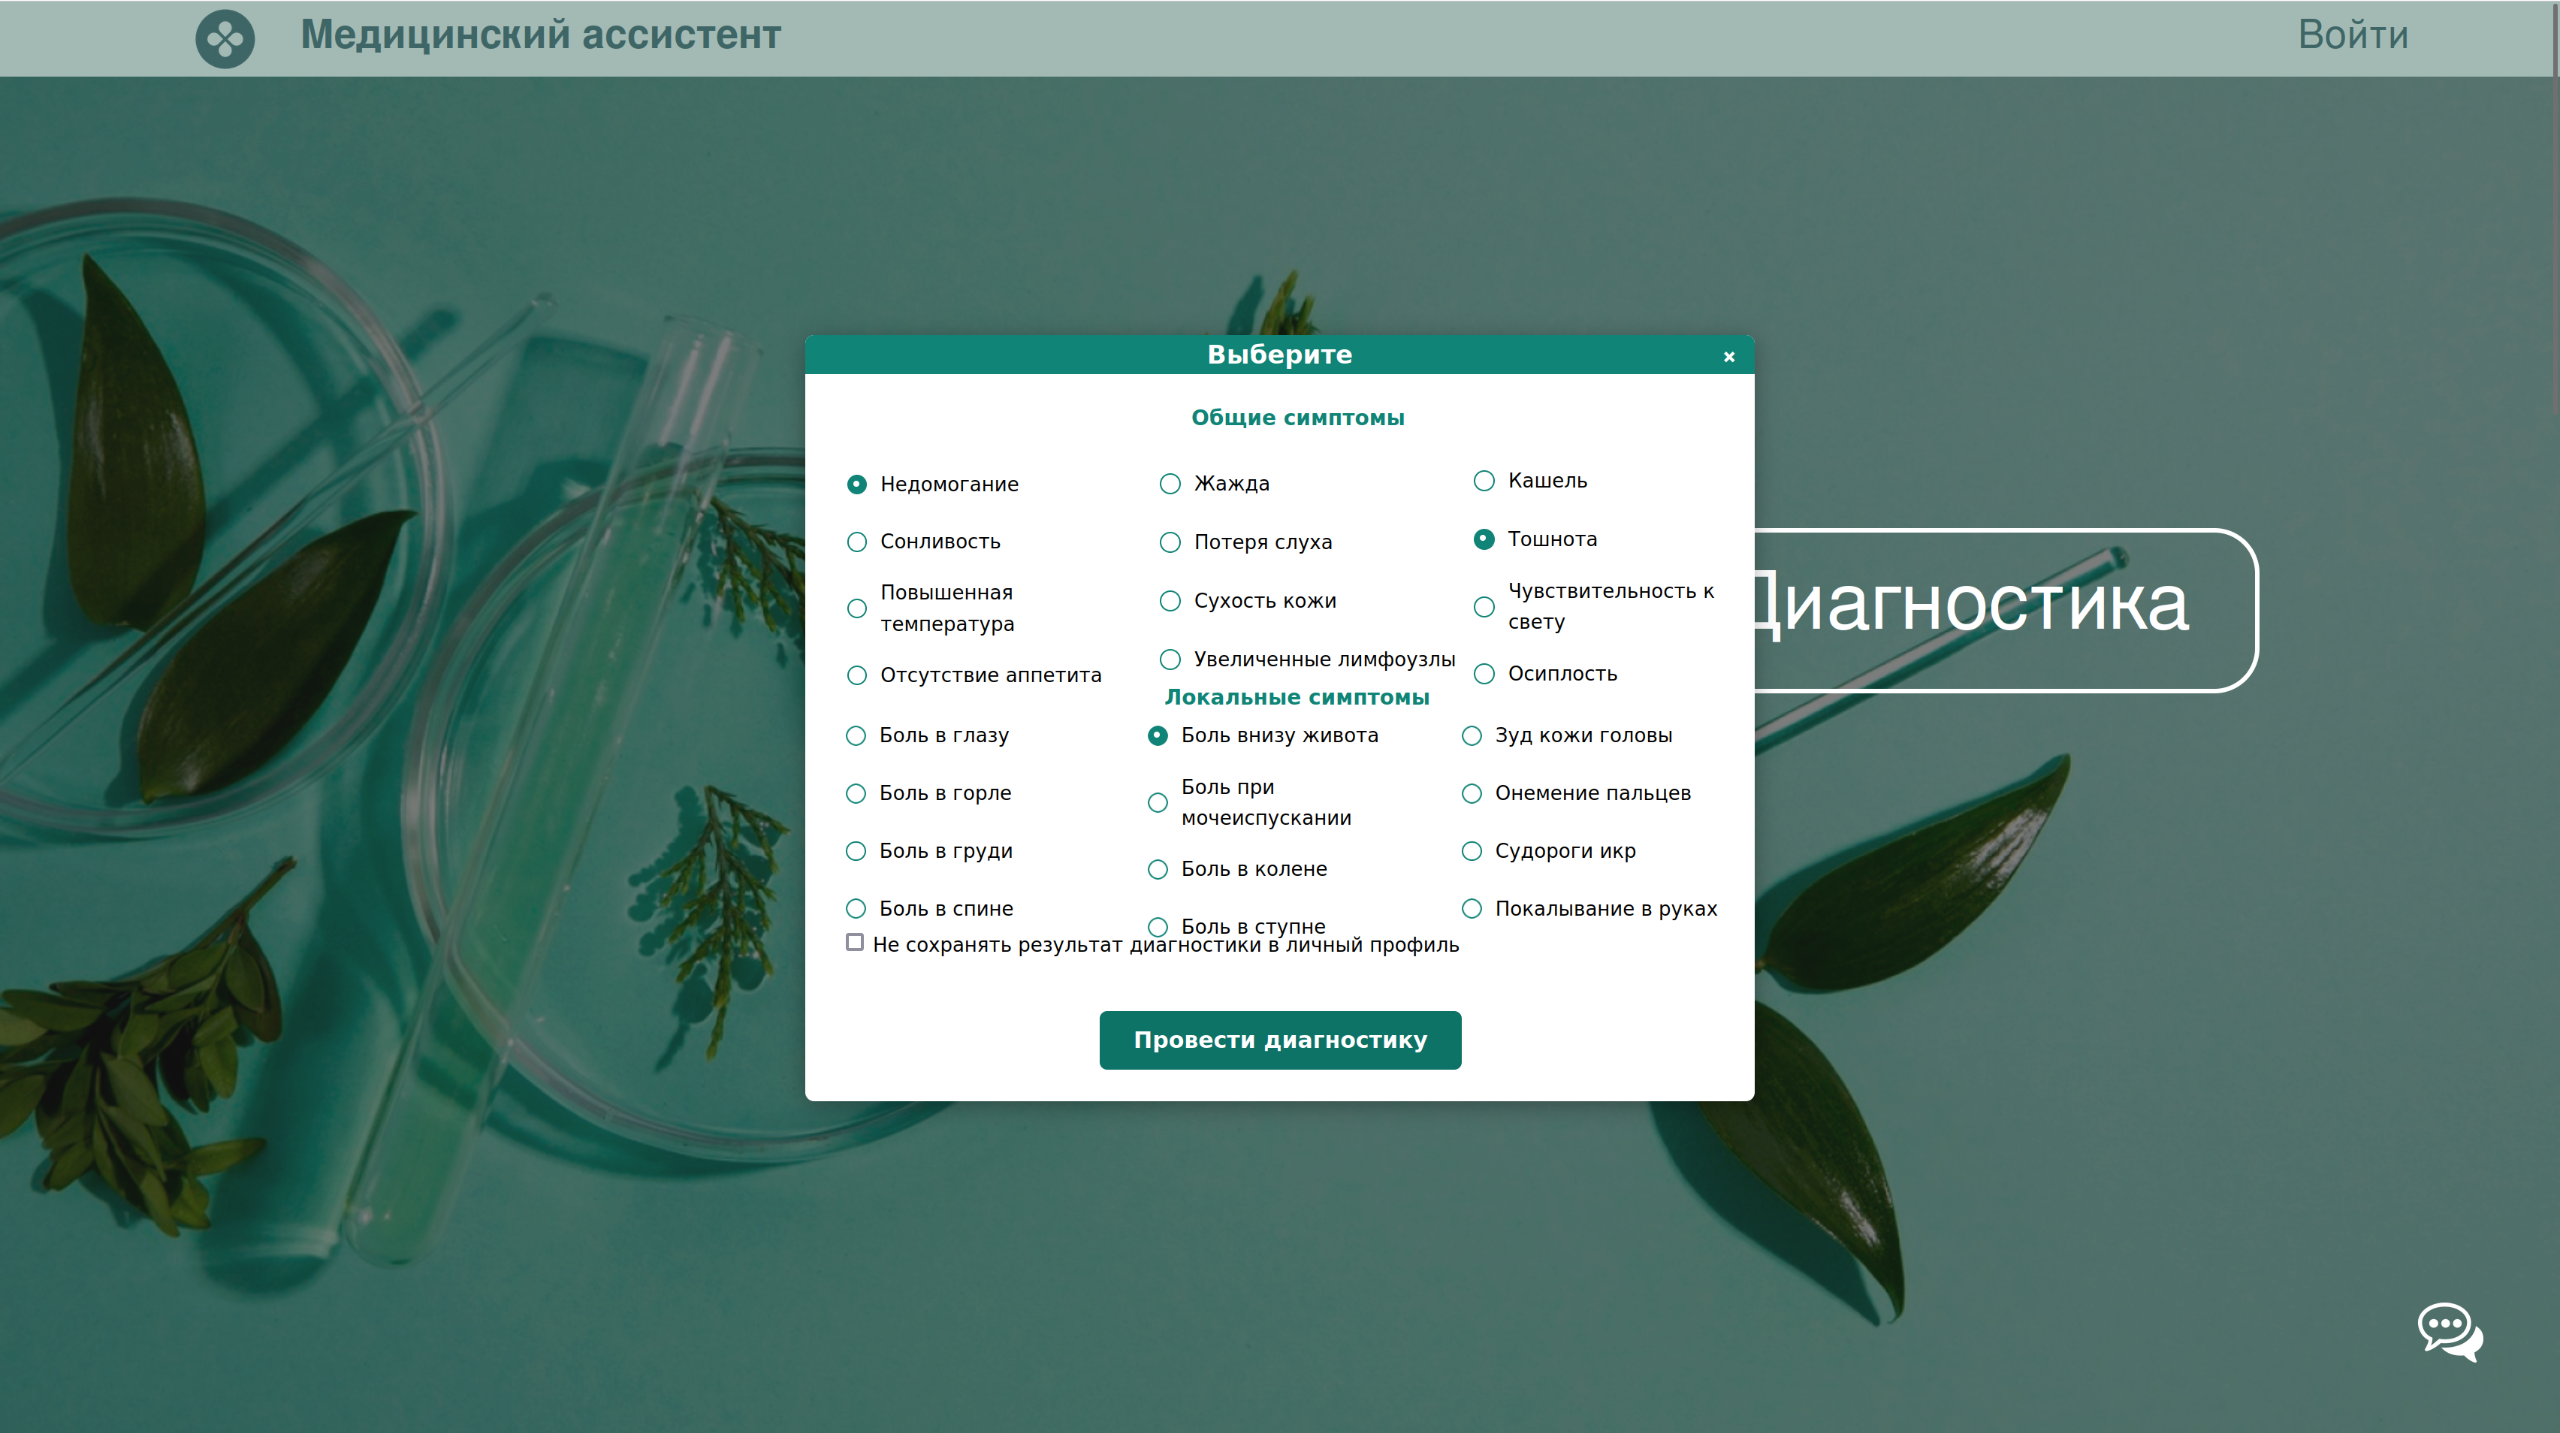
\includegraphics[width=0.9\textwidth]{sections/symptoms_diagnostic.png}
    \caption{Окно диагностики по симптомам}
    \label{симптомы}
\end{figure}

\begin{figure}[H]
    \centering
    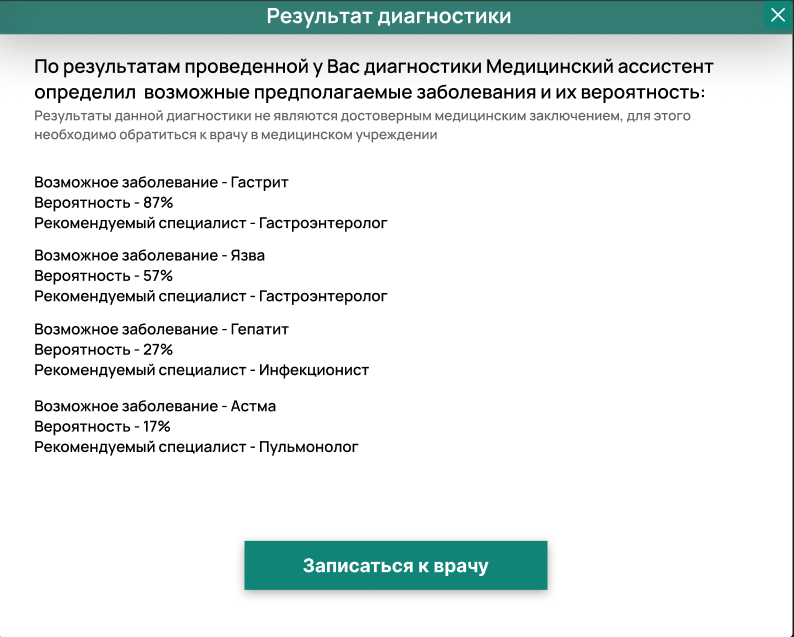
\includegraphics[width=0.9\textwidth]{sections/symptoms_result.png}
    \caption{Окно результата диагностики по симптомам}
    \label{симптомы_рузультат}
\end{figure}


\begin{figure}[H]
    \centering
    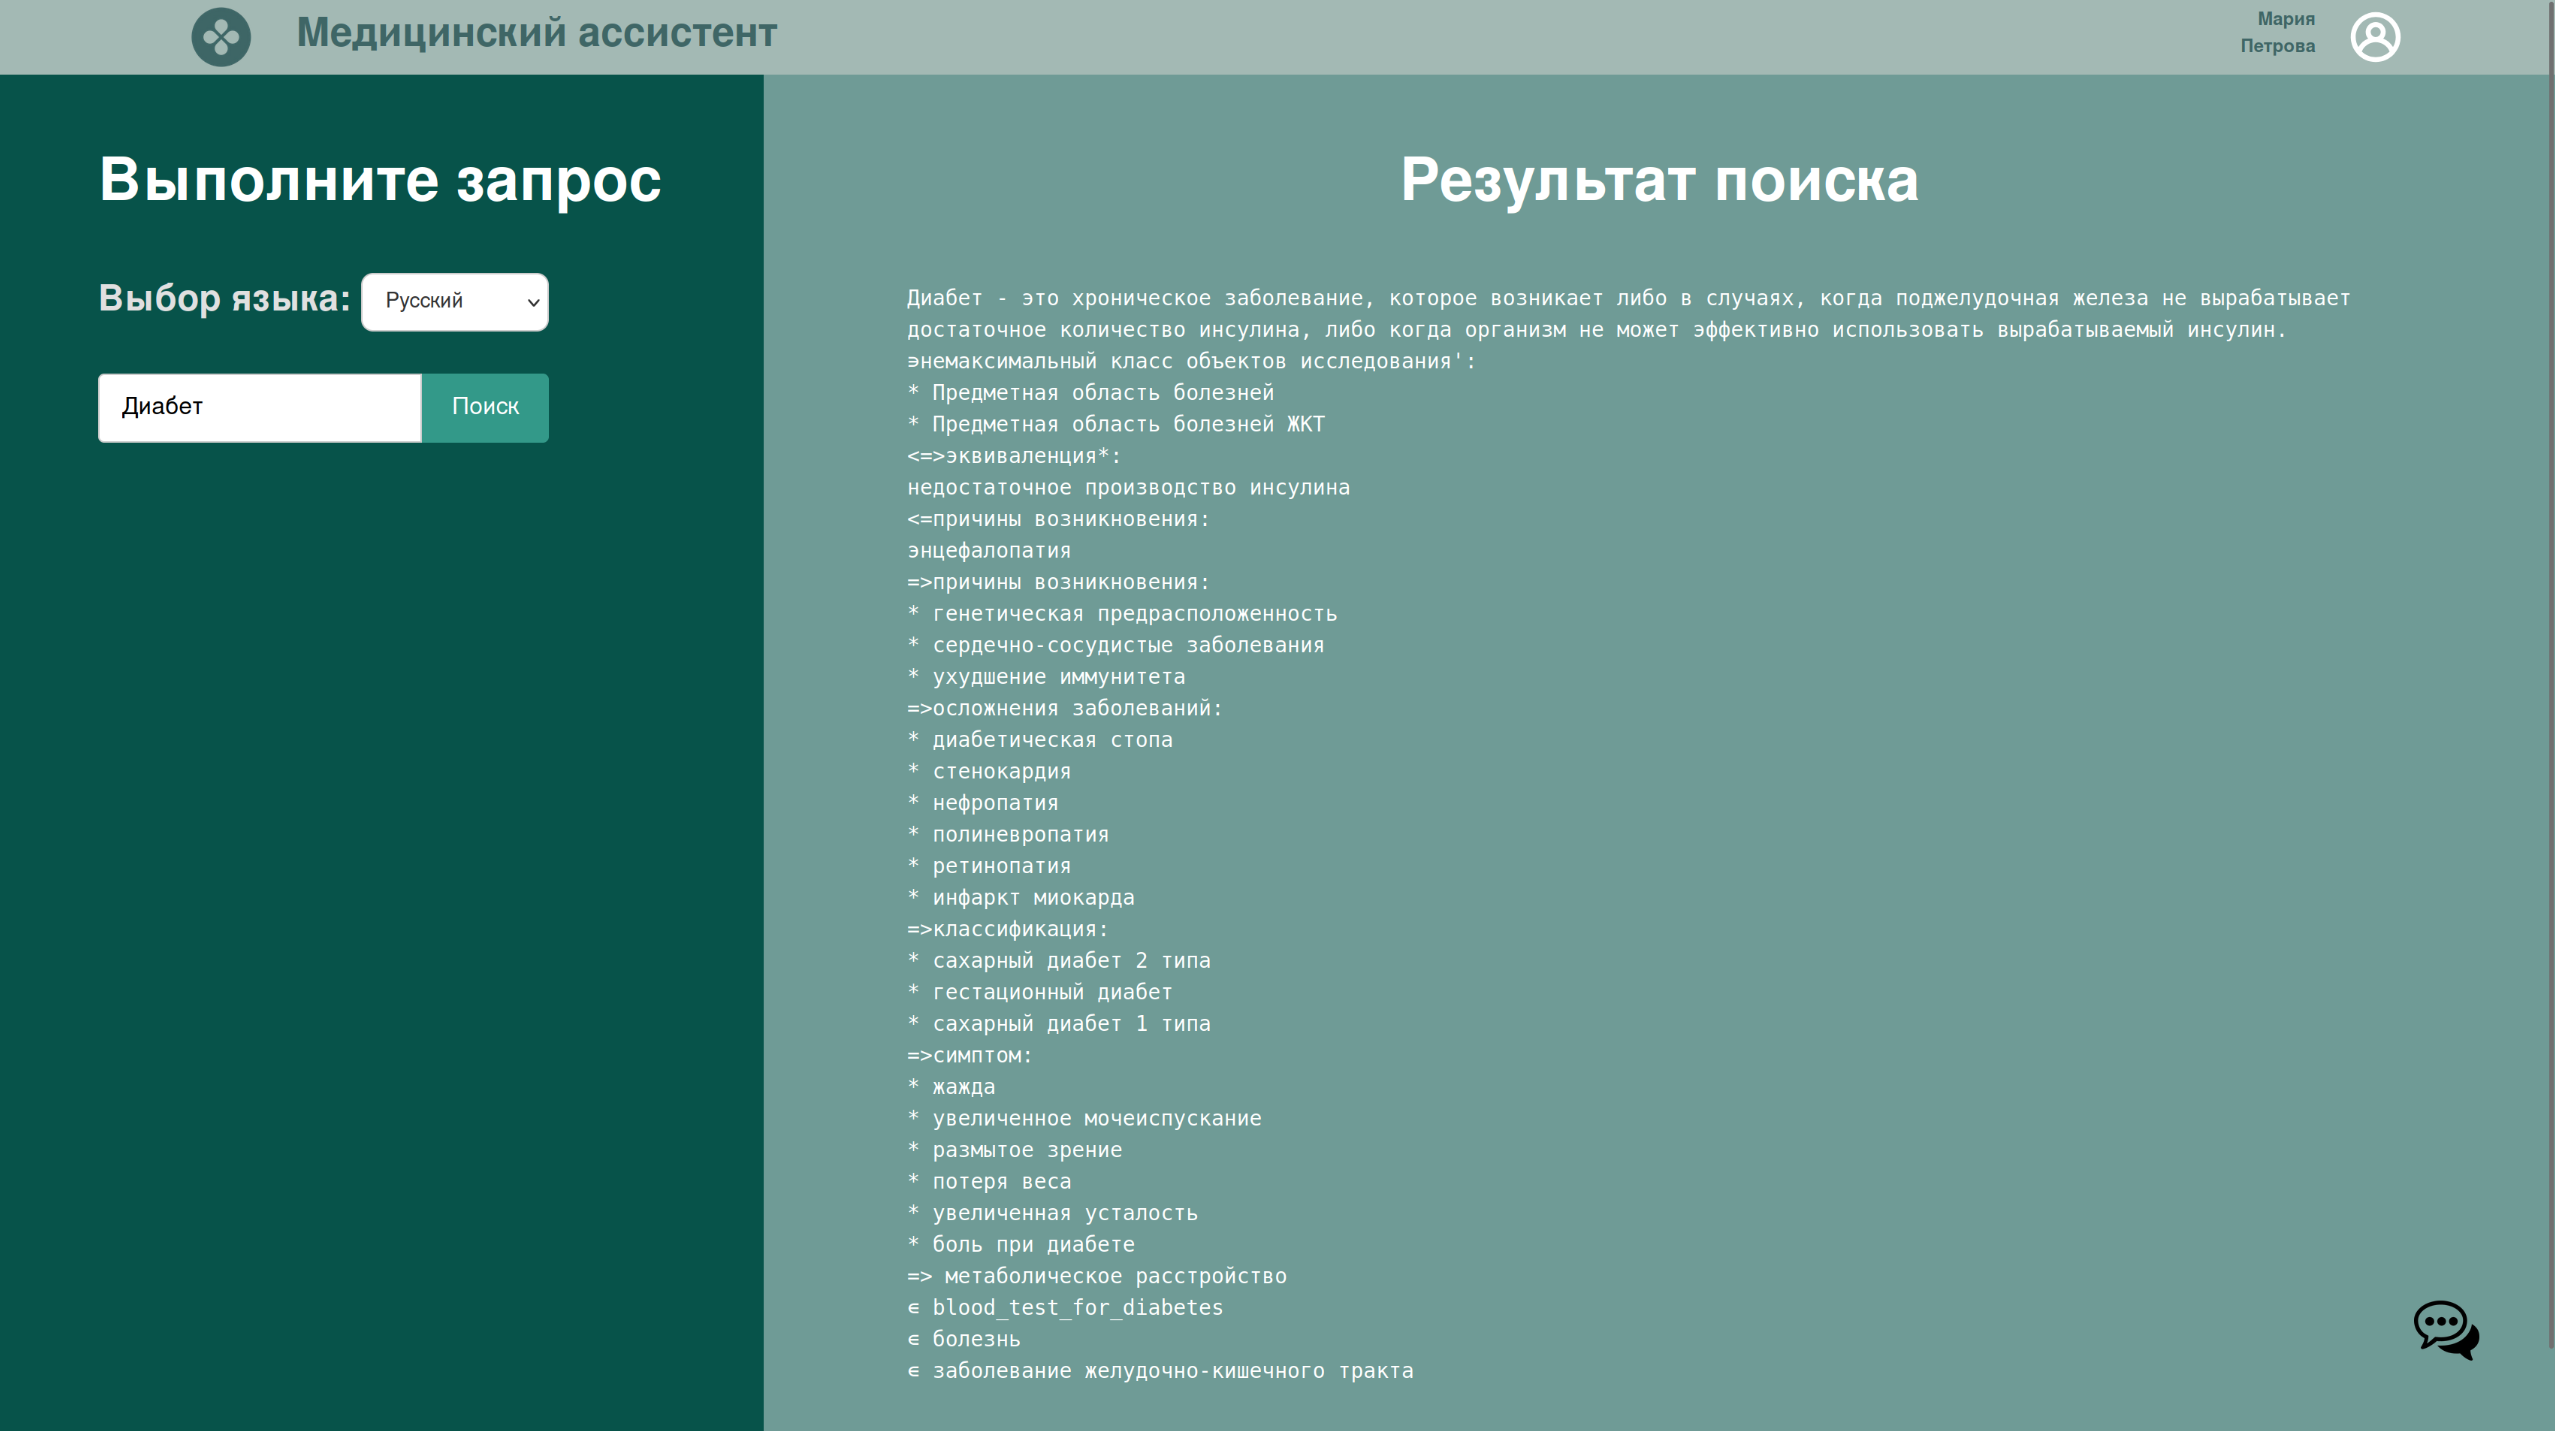
\includegraphics[width=0.9\textwidth]{sections/navigation_base.png}
    \caption{Окно с навигацией по базе знаний}
    \label{навигация}
\end{figure}

Были разработаны и интегрированы в веб-приложение чаты, включающие в себя функционал интеллекутального чата для для быстрых вопросов по истории болезней пациента и рекомендациям по здоровью без привлечения помощи медицинского персонала \hyperref[миничат]{3.19}, а также личный чат для обеспечения оперативной коммуникации между медицинским персоналом и пациентом в режиме реального времени \hyperref[личныйчат]{3.20}

\begin{figure}[H]
    \centering
    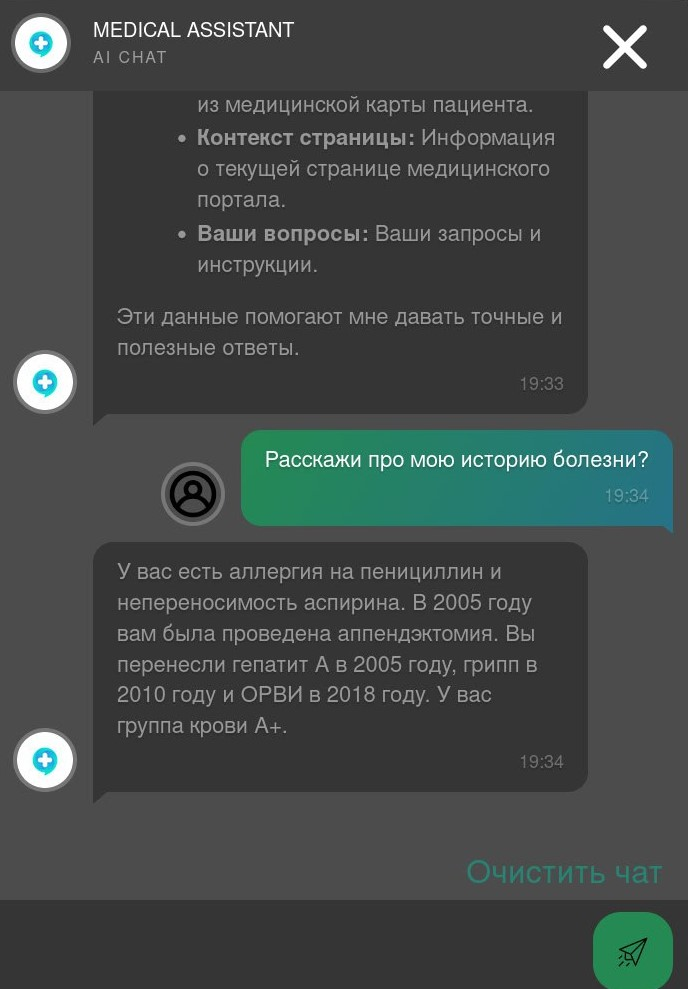
\includegraphics[width=0.9\textwidth]{sections/ai-chat.jpg}
    \caption{Интеллекутальный чата для для быстрых вопросов}
    \label{миничат}
\end{figure}

\begin{figure}[H]
    \centering
    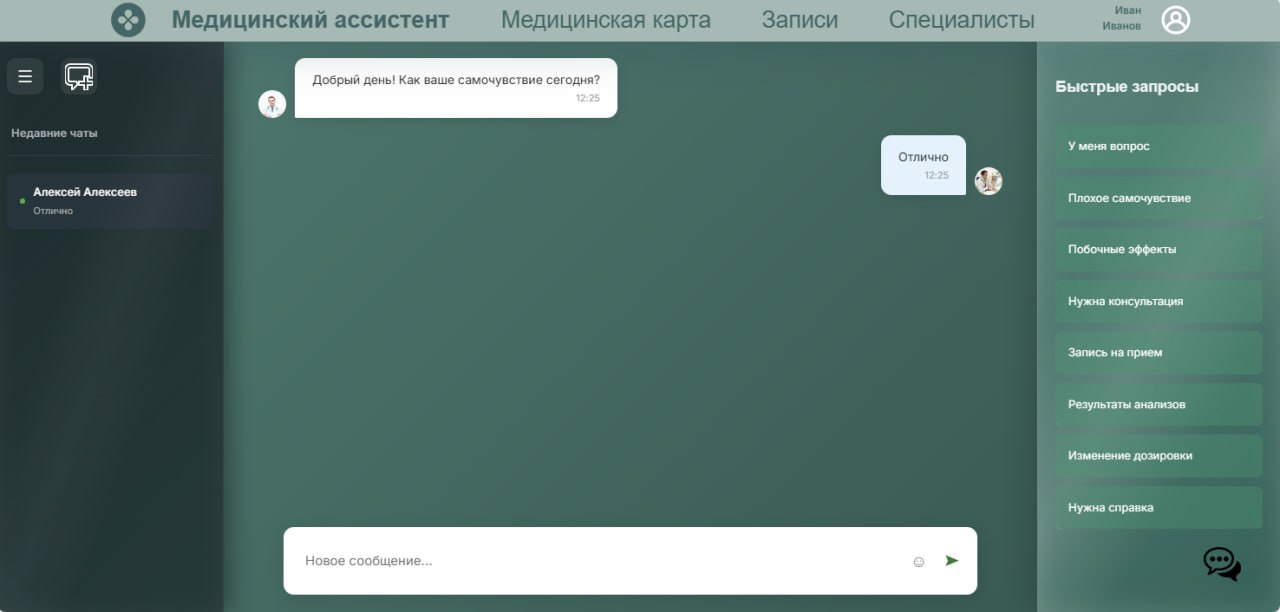
\includegraphics[width=0.9\textwidth]{sections/personal_chat.jpg}
    \caption{Страницы личных сообщений}
    \label{личныйчат}
\end{figure}

Также в хоже разработки приложения была интегрирована RAG система для загрузки  \hyperref[рагзагрузка]{3.21} и обработки \hyperref[рагобраюоткаа]{3.22} медицинских документов, а также созможности составления отчетов по состоянию здоровью пациента \hyperref[раготчет]{3.23}, дополнительно к этому был реализован функционал возможности использования диалогового окна для уточнения необходимых вопросов по содержанию загружаемых документов \hyperref[рагвопрос]{3.24}

\begin{figure}[H]
    \centering
    
\includegraphics[width=0.9\textwidth]{sections/rag_upload.jpg}
    \caption{Страницы загрузки медецинском документов}
    \label{рагзагрузка}
\end{figure}

\begin{figure}[H]
    \centering
    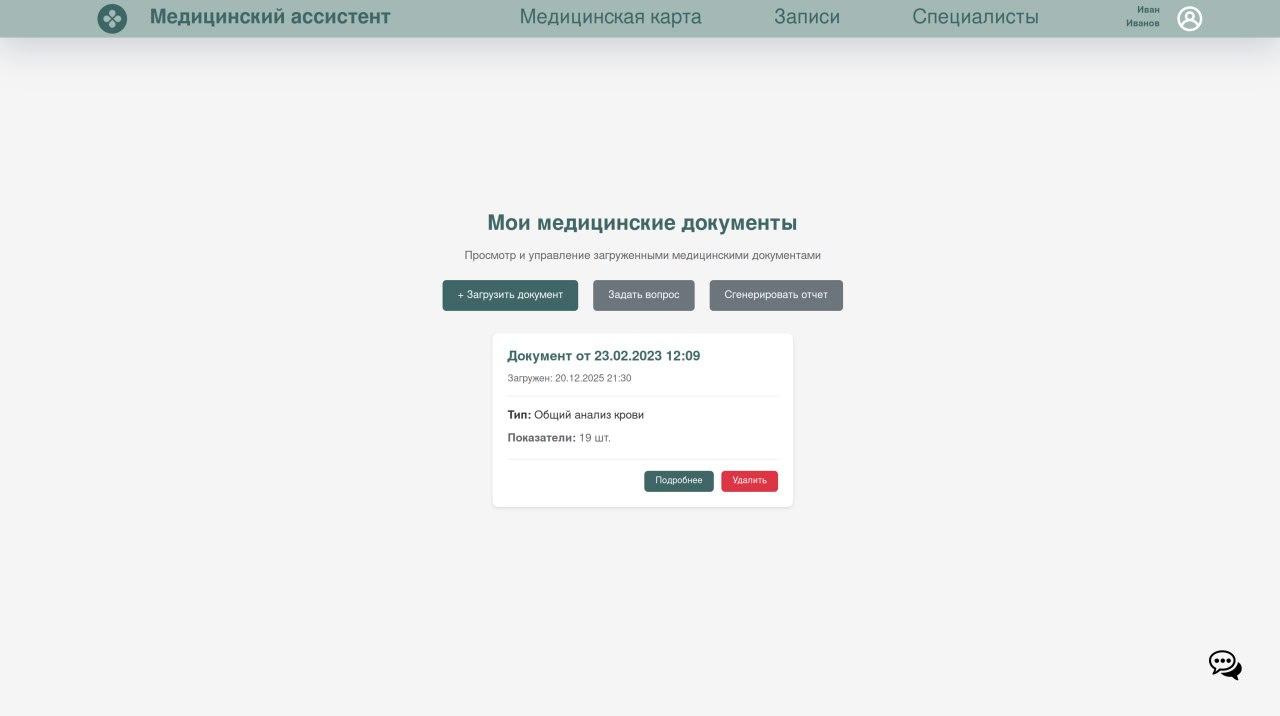
\includegraphics[width=0.9\textwidth]{sections/rag_processing.jpg}
    \caption{Страницы обработки медицинскоих документов}
    \label{рагобраюоткаа}
\end{figure}

\begin{figure}[H]
    \centering
    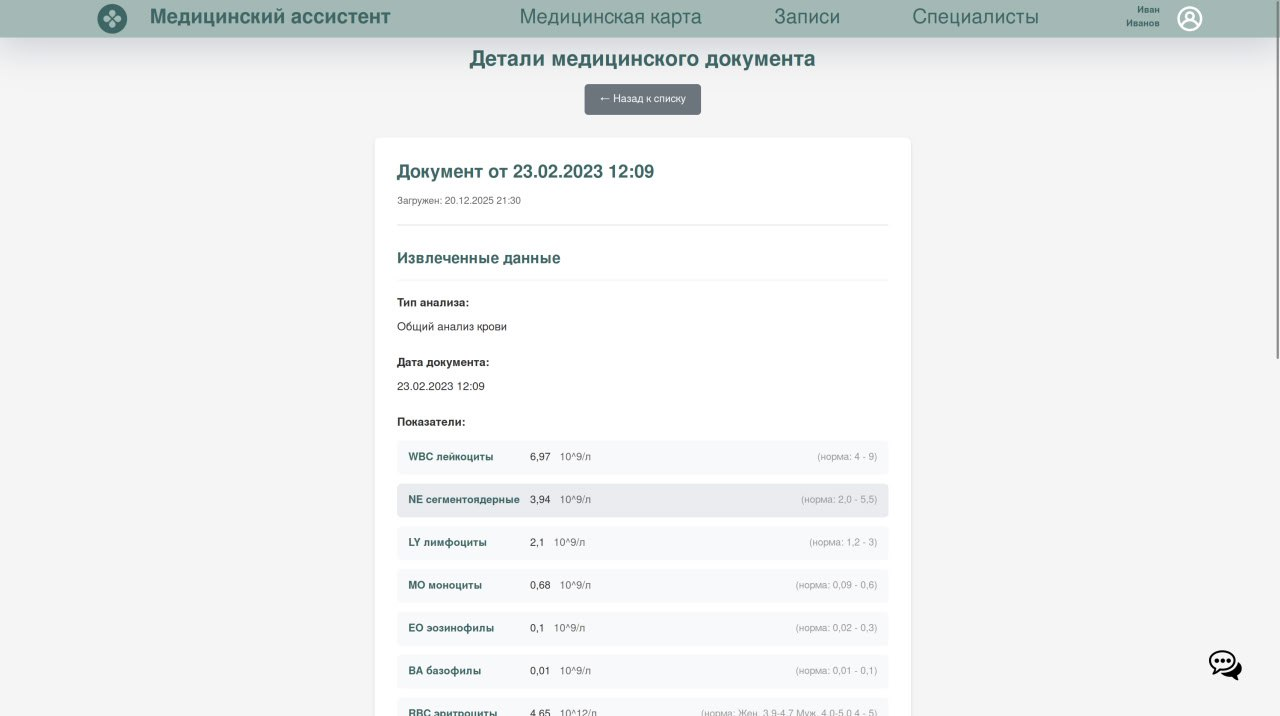
\includegraphics[width=0.9\textwidth]{sections/rag_report.jpg}
    \caption{Страницы отчета по загруженным документам}
    \label{раготчет}
\end{figure}

\begin{figure}[H]
    \centering
    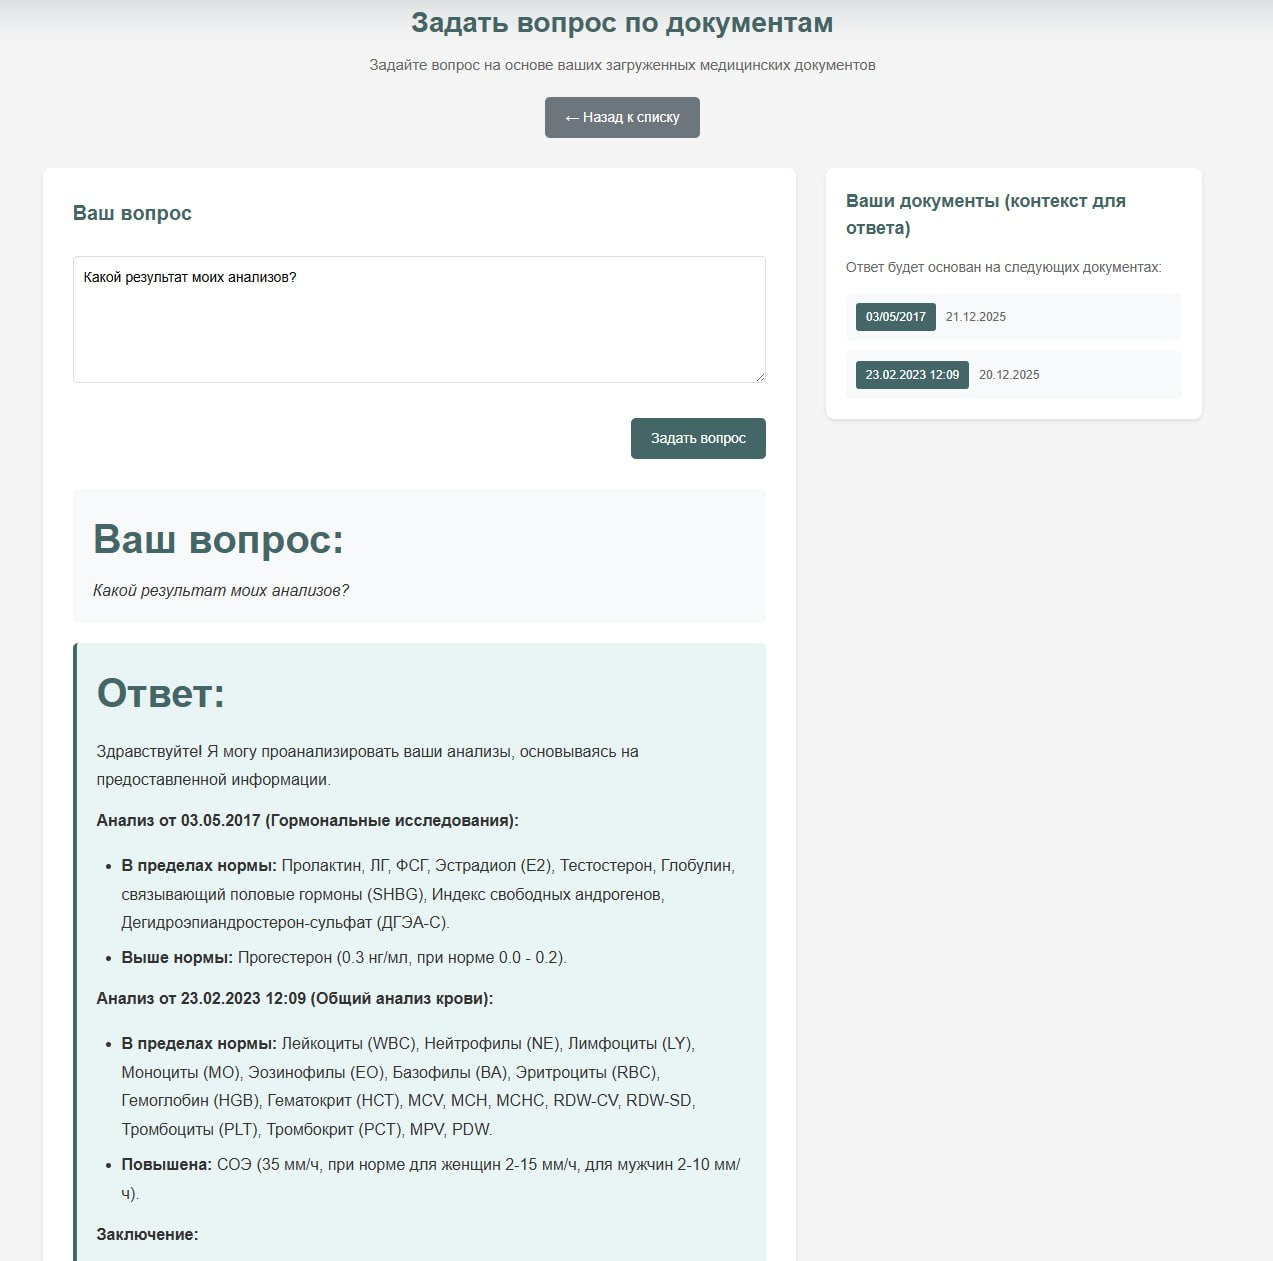
\includegraphics[width=0.9\textwidth]{sections/rag_chat.jpg}
    \caption{Страницы обработки вопросов на основе загруженных документов}
    \label{рагвопрос}
\end{figure}

В качетсве дополнительного функционала для регулярного обновления и актуализации данных о состоянии медицинских показателей здоровья пациента, возможности их дальнейшего прогнозирования, а также их первичной статистической обработки и предоставления лечащему врачу в удобном визуальном формате была реализована страница мониторинга состояния здоровья. Примеры работы представлены на рисунках \hyperref[статазапись]{3.25}, \hyperref[стататренд]{3.26} и \hyperref[статаграфики]{3.27}.

\begin{figure}[H]
    \centering
    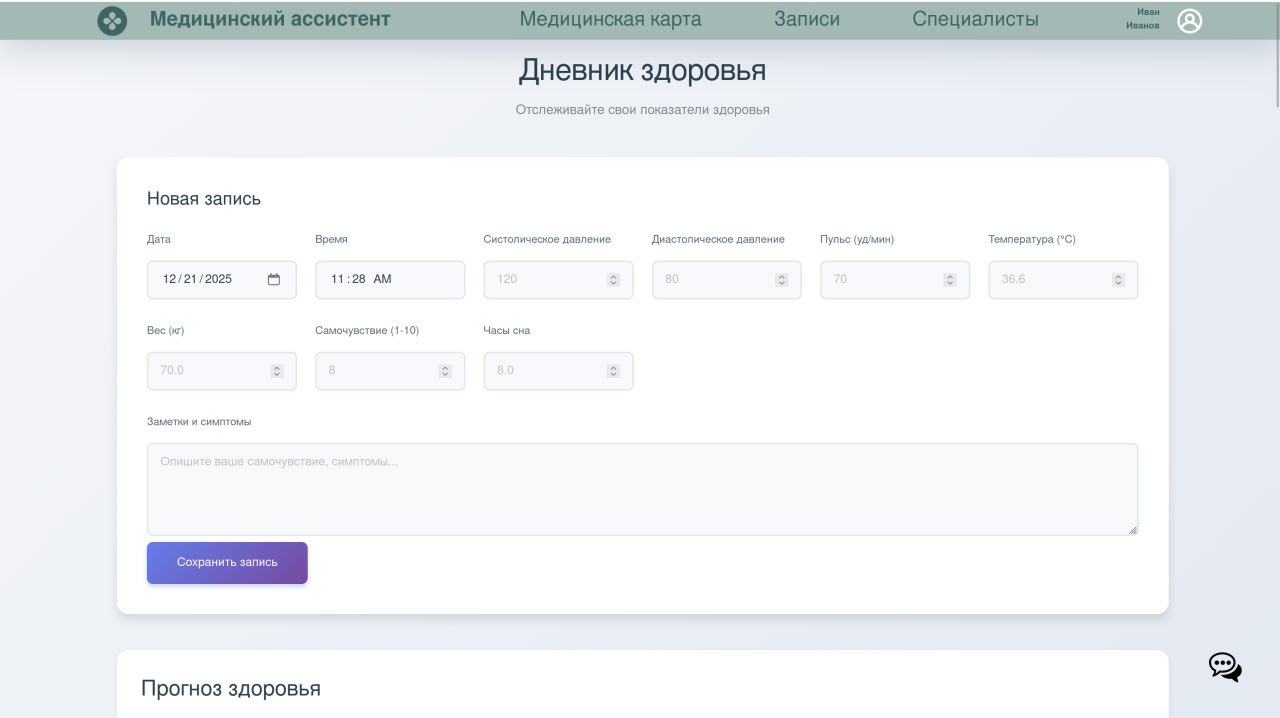
\includegraphics[width=0.9\textwidth]{sections/dairy_add.jpg}
    \caption{Окно добавления записи о текущем состоянии здоровья}
    \label{статазапись}
\end{figure}

\begin{figure}[H]
    \centering
    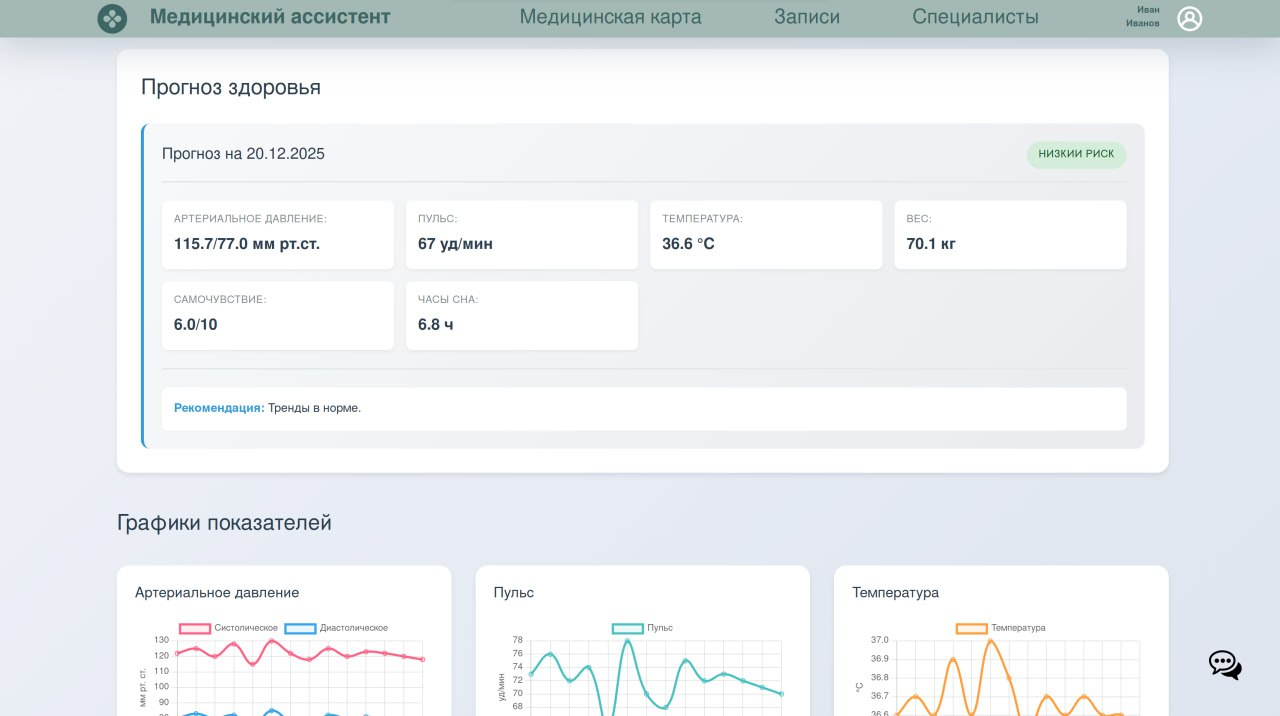
\includegraphics[width=0.9\textwidth]{sections/dairy_trend.jpg}
    \caption{Окно прогнозирования динамики дальнешего изменения состояни здоровья}
    \label{стататренд}
\end{figure}

\begin{figure}[H]
    \centering
    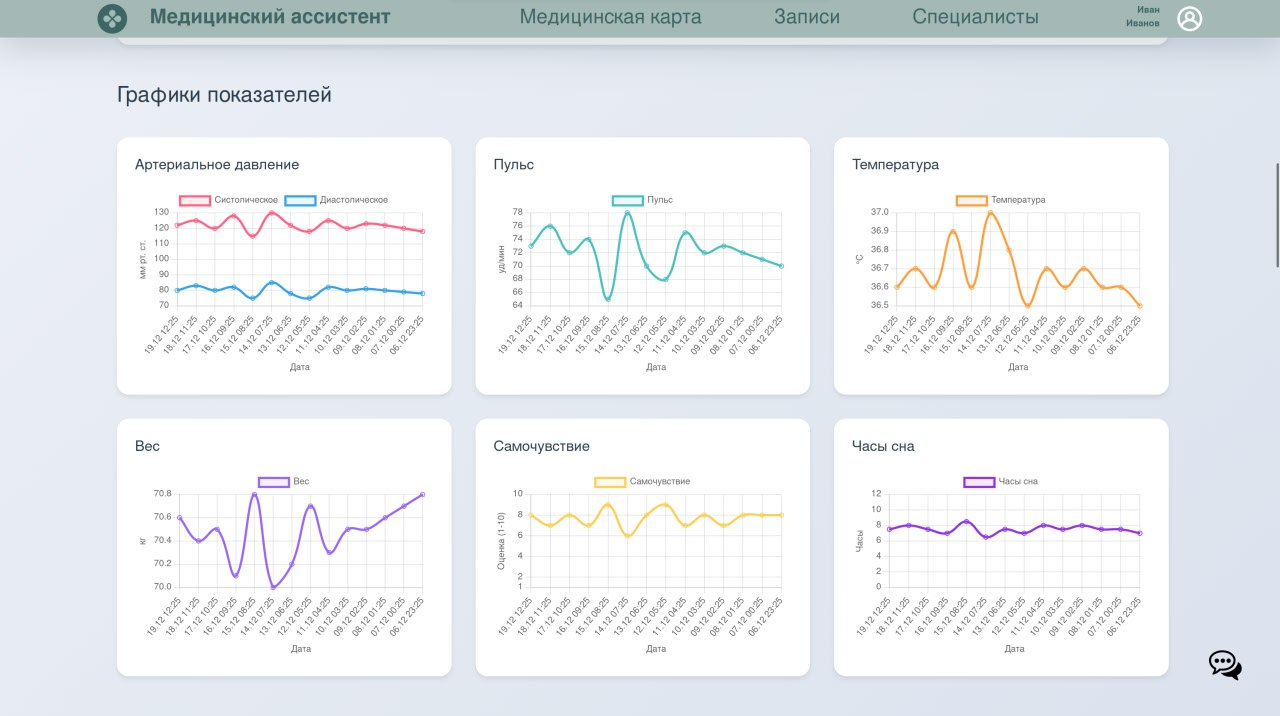
\includegraphics[width=0.9\textwidth]{sections/dairy_graphics.jpg}
    \caption{Набор графиков изменения показателей для быстрой первичной статистической обработки}
    \label{статаграфики}
\end{figure}

\subsection{Вывод}

В данном разделе были выделены и описаны основные инструменты, используемые в ходе разработки интеллектуальной медицинской системы. Среди них были выделены следующие ключевые компоненты:

\begin{itemize}
    \item метасистема OSTIS — универсальная основа для проектирования интеллектуальных систем, обеспечивающая высокую гибкость, адаптивность и совместимость.
    \item Docker — платформа для контейнеризации, позволяющая развертывать приложения на различных операционных системах, обеспечивая простоту распространения и использования.
    \item Python — высокоуровневый язык программирования с широким набором библиотек, подходящий для реализации интеллектуальных систем и работы с данными.
\end{itemize}

Данные инструменты обеспечивают надежную основу для реализации интеллектуальной медицинской системы, обеспечивая необходимые функциональные возможности и технические характеристики для дальнейшего тестирования и эксплуатации разрабатываемой системы.

